\documentclass{article}
\usepackage{graphicx} % Required for inserting images
\usepackage{enumerate} %makes numbered lists
\usepackage{setspace}
\usepackage[hidelinks]{hyperref}
\usepackage{epsfig}  % for figures
\usepackage{url}  % Hyphenation of URLs.
\usepackage{lscape}  % Useful for wide tables or figures.
\usepackage[justification=raggedright]{caption}	% makes captions ragged right - thanks to Bryce Lobdell
\usepackage[labelfont=bf]{caption} % Makes the FIGURE X part of the figure caption bold
\usepackage{array} % For tables
\usepackage{multirow} %Merge multiple rows in tables
\usepackage{hhline} % for underlining table cells
\usepackage{framed} % frame around all subfigures
\usepackage{adjustbox} % custom frame around all subfigures
\usepackage{float}
\usepackage{booktabs}
\usepackage{amsmath}  % for math spacing
\usepackage{xcolor, soul} %lets us change the text color
\usepackage{enumerate}

\usepackage{geometry}
 \geometry{
 a4paper,
 total={170mm,257mm},
 left=20mm,
 top=20mm,
 }

%Commands to make the text red or blue
\newcommand{\red}[1]{\textcolor{red}{#1}}
\newcommand{\blue}[1]{\textcolor{blue}{#1}}

\title{MechSE Web Reference Page - TAM 210}
%\author{Updated}

\begin{document}

\maketitle
\date


\blue{Blue text:} Notes to whoever is transcribing these reference pages to the website

\red{Red text:} Unfinished secitons / questions

\tableofcontents

\newpage

%Add new topics by copying the topic.tex file - you should rename it to be more specific to your course. 
\section{Introduction to Statics}

\subsection{Newton's Laws}

\blue{From TAM212 Reference Pages (Kinetics of Point Masses - Newton's Equations):}


Newton's equations relate the acceleration $\vec{a}$ of a point mass with mass $m$ to the total applied force $\vec{F}$ on the mass (sum of all applied forces). There is no derivation for Newton's equations, because they are an assumed model for dynamics. We can only verify them by comparing with experimental evidence, which confirms that Newtonian dynamics are accurate for non-relativistic and non-quantum systems.

They are:

\subsubsection{Newton's First Law}

A particle at rest stays that way unless acted on by unbalanced forces. 

\subsubsection{Newton's Second Law}

\[\vec{F} = m \vec{a}\]

\subsubsection{Newton's Third Law}

The mutual forces of action and reaction between two particles are equal, opposite, and collinear. 

\subsubsection{Example}

\begin{figure*}[!h]
\centering
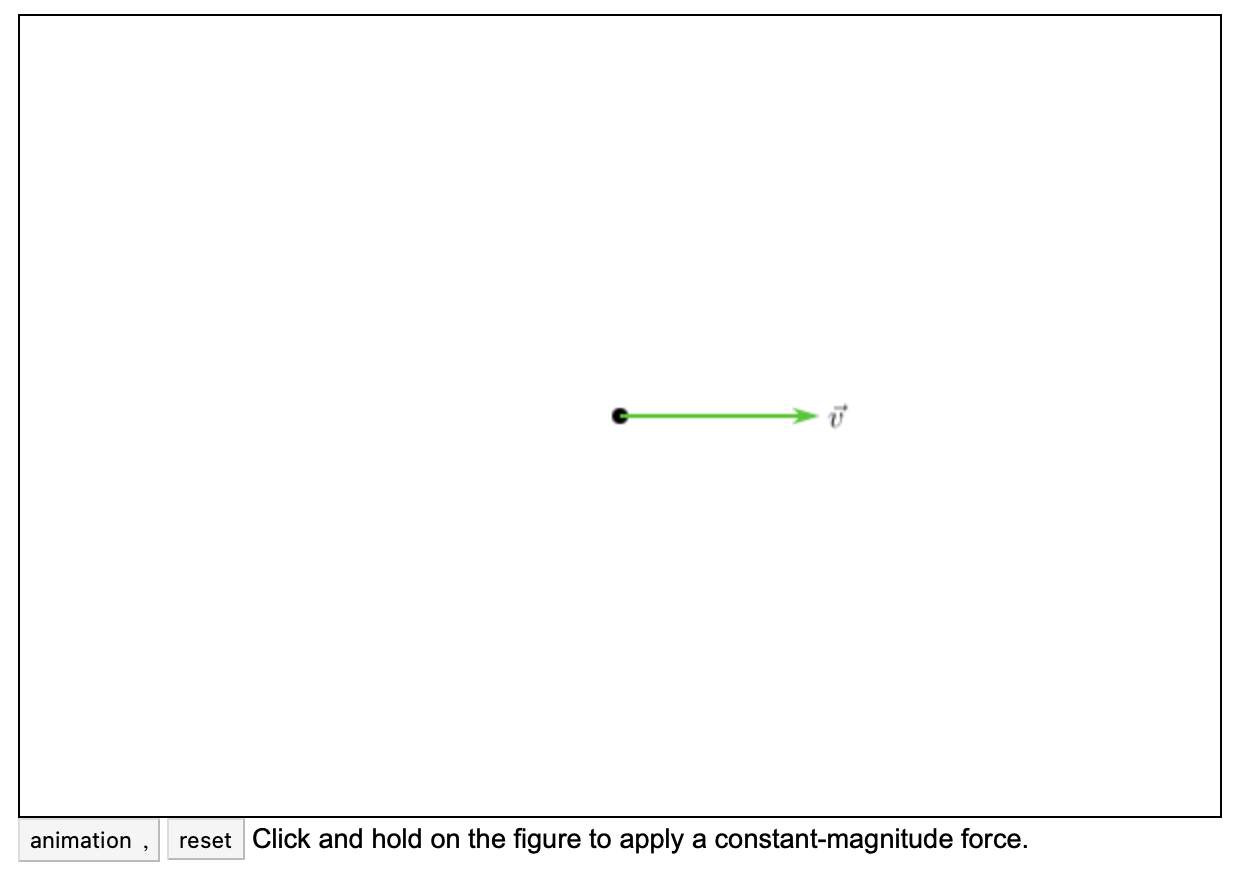
\includegraphics[angle=0, width=5in]{IntroductionFigures/NewtonsLaws.png}
\vspace{-2mm}
\caption{\small \blue{Taken from TAM212 Reference Pages (Kinetics of Point Masses - Newton's Equations)}}
\vspace{-3mm}
\label{Fig:NewtonsLaws}
\end{figure*}

\subsection{Idealizations}

\subsubsection{Particles}
%Could change this section to "Idealizations" and write about particle idealizations, rigid body assumptions, and concentrated / distributed force assumptions. 

In this course, we assume two things about particles: 

\begin{enumerate}
    \item{The mass of the particle is not 0.}
    \item{The radius of the mass is 0.}
\end{enumerate}

\noindent Through these assumptions, we are essentially concentrating all of the mass of an object at a single point in space. The particle has a mass but the size and shape of the particle is not taken into account. 

\subsubsection{Rigid Bodies}

For rigid bodies, we assume that the object has both mass (similar to particles) but also take its shape into account. 

We call these bodies "rigid" because we assume that they do not deform under applied forces or moments. 

\blue{Insert the same content here as from the TAM212 Reference Pages (Rigid Bodies - introductory section at the top of the page).}


\section{Cartesian Coordinates}

\blue{Insert the same content here as from the TAM212 Reference Pages (Positions and Coordinates - Cartesian Coordinates)}

\subsection{Vector Bases}

\blue{Insert the same content here as from the TAM212 Reference Pages (Vectors and Bases - Vector Bases)}

\subsection{Right Hand Rule}

The Cartesian system is a "right-handed" coordinate system, which means that we can use the right-hand rule to determine the direction of the $x, y$ and $z$ axes. In 3D the $x, y, z$ axes are oriented in right-handed order, so that fingers curling from $x$ to $y$ means the thumb points in the $z$ direction.

\begin{figure*}[!h]
\centering
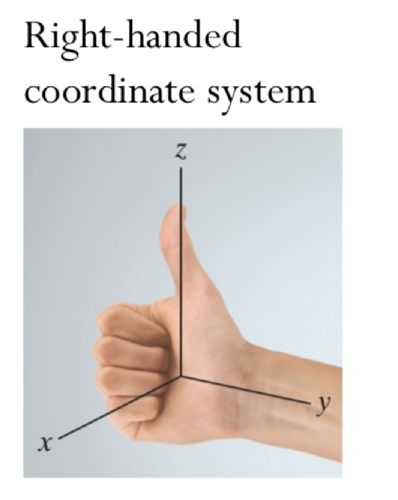
\includegraphics[angle=0, width=2in]{CartCoordFigures/RightHandRule.png}
\vspace{-2mm}
\caption{\small \blue{Taken from TAM 210 Lecture 3 - Slide 3}}
\vspace{-3mm}
\label{Fig:NewtonsLaws}
\end{figure*}



\section{Vectors and Scalars}

%\subsection{Force Vectors}

%I'm not sure we need a reference page for this - or maybe put it at the end?

\subsection{Scalars vs. Vectors}

\subsubsection{Vectors}

\blue{From TAM212 Reference Pages (Vectors and Bases):}

A \textit{vector} is an arrow with a length and a direction. Just like positions, vectors exist before we measure or describe them. Unlike positions, vectors can mean many different things, such as position vectors, velocities, etc. Vectors are not anchored to particular positions in space, so we can slide a vector around and locate it at any position.

\begin{figure*}[!h]
\centering
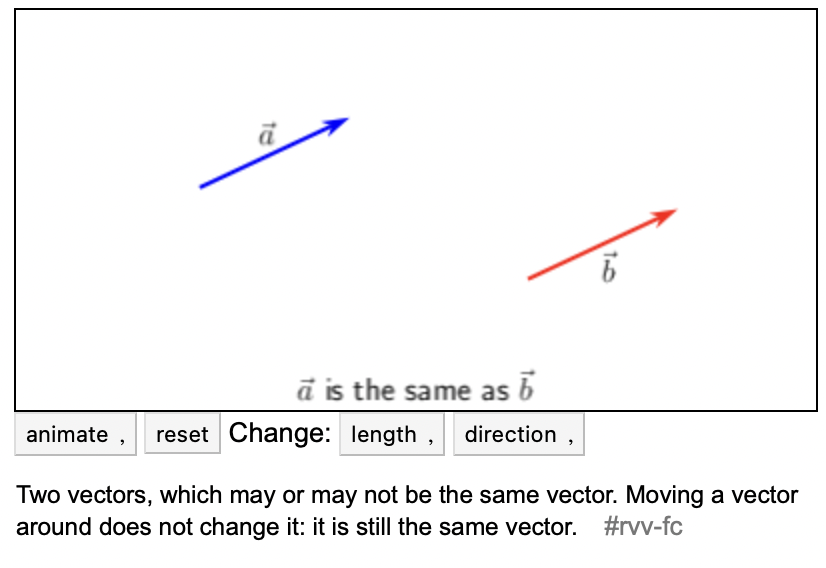
\includegraphics[angle=0, width=4in]{VectorsScalarsFigures/VectorDef.png}
\vspace{-2mm}
\caption{\small \blue{Taken from TAM212 Reference Pages (Vectors and Bases)}}
\vspace{-3mm}
\label{Fig:NewtonsLaws}
\end{figure*}

\subsubsection{Scalars}

While a vector represents magnitude and direction, a \textit{scalar} is a number that represents a magnitude, but with no directional information. Some examples of scalar quantities can be mass, length, time, speed, or temperature. 

\subsection{Vector Operations}

\subsubsection{Scaling Vectors}

\blue{Taken from TAM212 Reference Pages (Vectors and Bases)}

Vectors can be multiplied by a scalar number, which multiplies their length. 

\begin{figure*}[!h]
\centering
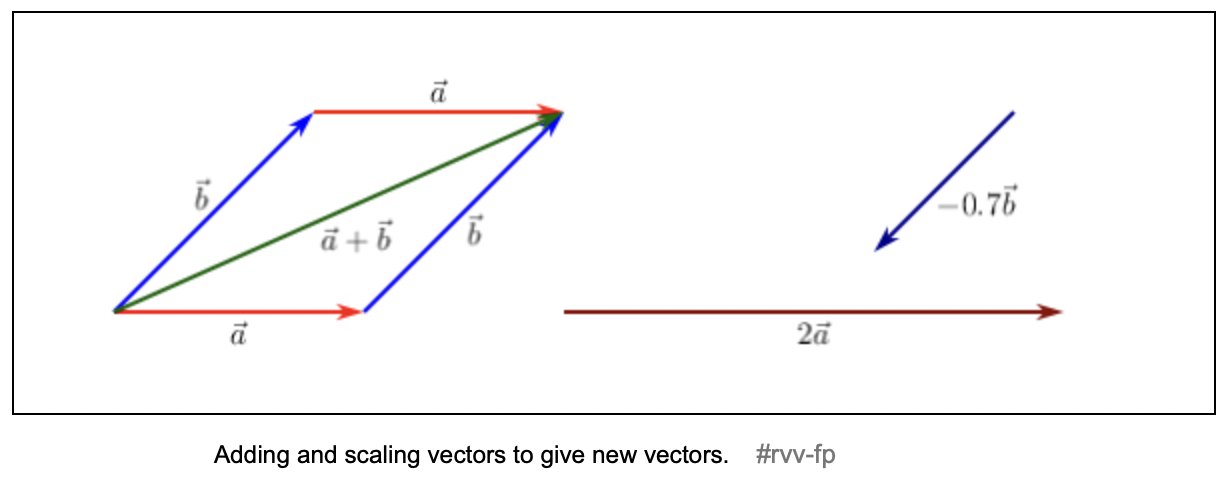
\includegraphics[angle=0, width=4in]{VectorsScalarsFigures/VecScaling.png}
\vspace{-2mm}
\caption{\small \blue{Taken from TAM212 Reference Pages (Vectors and Bases). Don't include the a+b vector - only keep one a and one b vector with their scaled counterparts.}}
\vspace{-3mm}
\label{Fig:NewtonsLaws}
\end{figure*}

\subsubsection{Vector Addition and Subtraction}

\blue{From TAM212 Reference Pages (Vectors and Bases):}

Vectors can be added or subtracted together, using the parallelogram law of addition or the head-to-tail rule.

\begin{figure*}[!h]
\centering
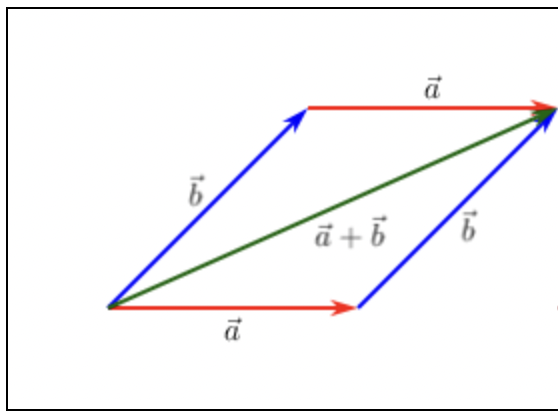
\includegraphics[angle=0, width=2in]{VectorsScalarsFigures/VecAddition.png}
\vspace{-2mm}
\caption{\small \blue{Taken from TAM212 Reference Pages (Vectors and Bases). Only include the left part of the figure, and add another part on the right that shows a-b.}}
\vspace{-3mm}
\label{Fig:NewtonsLaws}
\end{figure*}

\subsection{Unit Vectors}

\blue{Use the same content here as from the TAM212 Reference Pages (Vectors and Bases - Unit Vectors)}

\subsection{Vector Magnitude and Direction}

Vectors can be written as a magnitude (length) multiplied by the unit vector in the same direction as the original vector. 

\[\vec{A} = \|\vec{A}\|  \hat{u_A}\]

\blue{Insert the same content here as from the TAM212 Reference Pages (Vectors and Bases - Length of Vectors) for vector magnitude.}

The direction of a vector can be written as a unit vector by dividing the vector components by the vector magnitude. 

\begin{figure*}[!h]
\centering
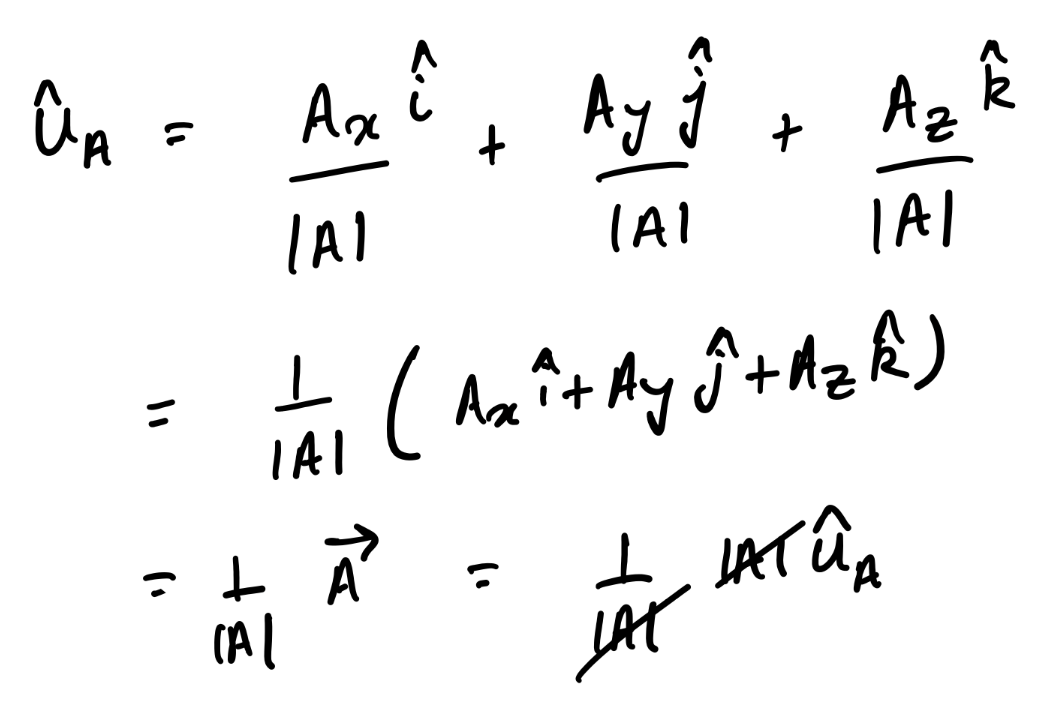
\includegraphics[angle=0, width=2in]{VectorsScalarsFigures/UnitVec.png}
\vspace{-2mm}
\caption{\small \blue{Taken from TAM210 Lecture Notes - Slide 3}}
\vspace{-3mm}
\label{Fig:NewtonsLaws}
\end{figure*}

Alternatively, the vector components can be determined geometrically via the angles of each component with respect to the Cartesian coordinates. 

\blue{Can probably make some sort of interactive figure here based on the image from TAM 210 lecture notes - slide 4}

\begin{figure*}[!h]
\centering
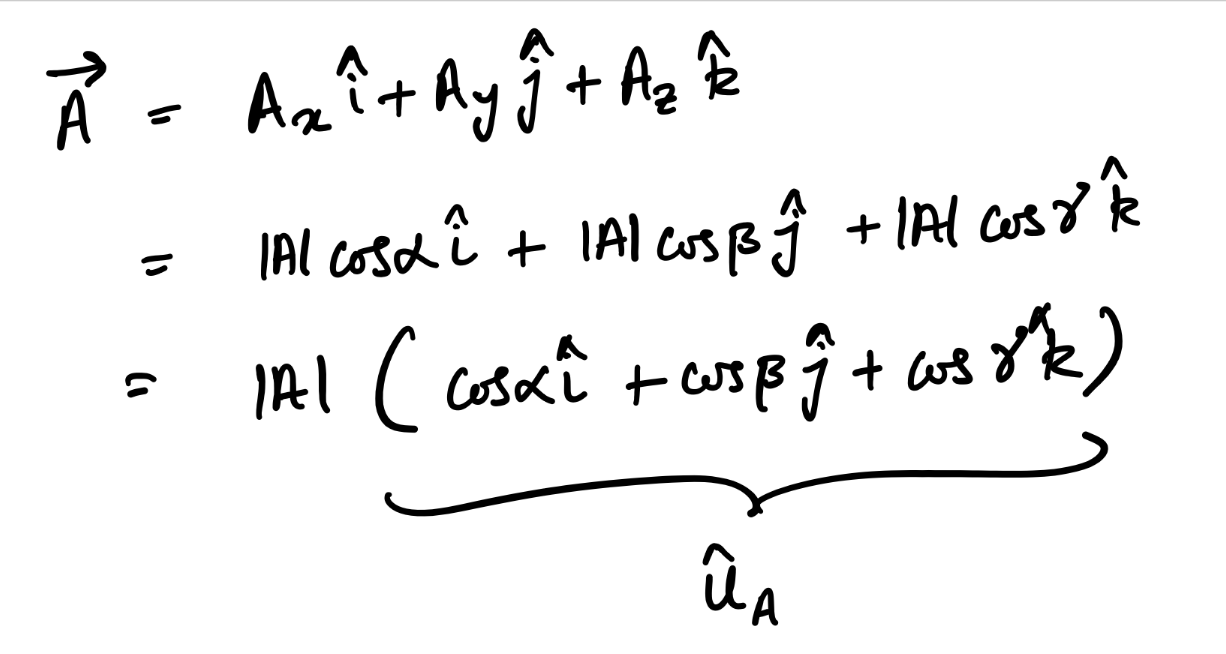
\includegraphics[angle=0, width=3in]{VectorsScalarsFigures/UnitVecAngles.png}
\vspace{-2mm}
\caption{\small \blue{Taken from TAM210 Lecture Notes - Slide 4}}
\vspace{-3mm}
\label{Fig:NewtonsLaws}
\end{figure*}


\subsection{Scalar and Vector Products}

\subsubsection{Dot Product}

\blue{Insert the same content here as from the TAM212 Reference Pages (Vectors and Bases - Dot Product).}

\subsubsection{\red{Cross Product}}

\red{Add something here about the three dimensional cross product?}

\blue{Insert the same content here as from the TAM212 Reference Pages (Vectors and Bases - Cross Product).}

\subsubsection{Vector Projection}

\blue{Insert the same content here as from the TAM212 Reference Pages (Vectors and Bases - Projection and Complementary Projection).}



\section{Free Body Diagrams}

\blue{Insert the same content here as from the TAM212 Reference Pages (Free Body Diagrams - the top introduction section). Note that if you try to click on the link to "Free Body Diagrams" from the TAM 210 reference page it doesn't work. You have to go into the TAM 212 reference page to access Free Body Diagrams. }

\subsection{Pulley Idealizations}

In this course we assume that a pulley is frictionless, meaning that the magnitude of the tensile force of the rope on either side of a pulley will be the same. 

\[{T_1} = {T_2}\]

\begin{figure*}[!h]
\centering
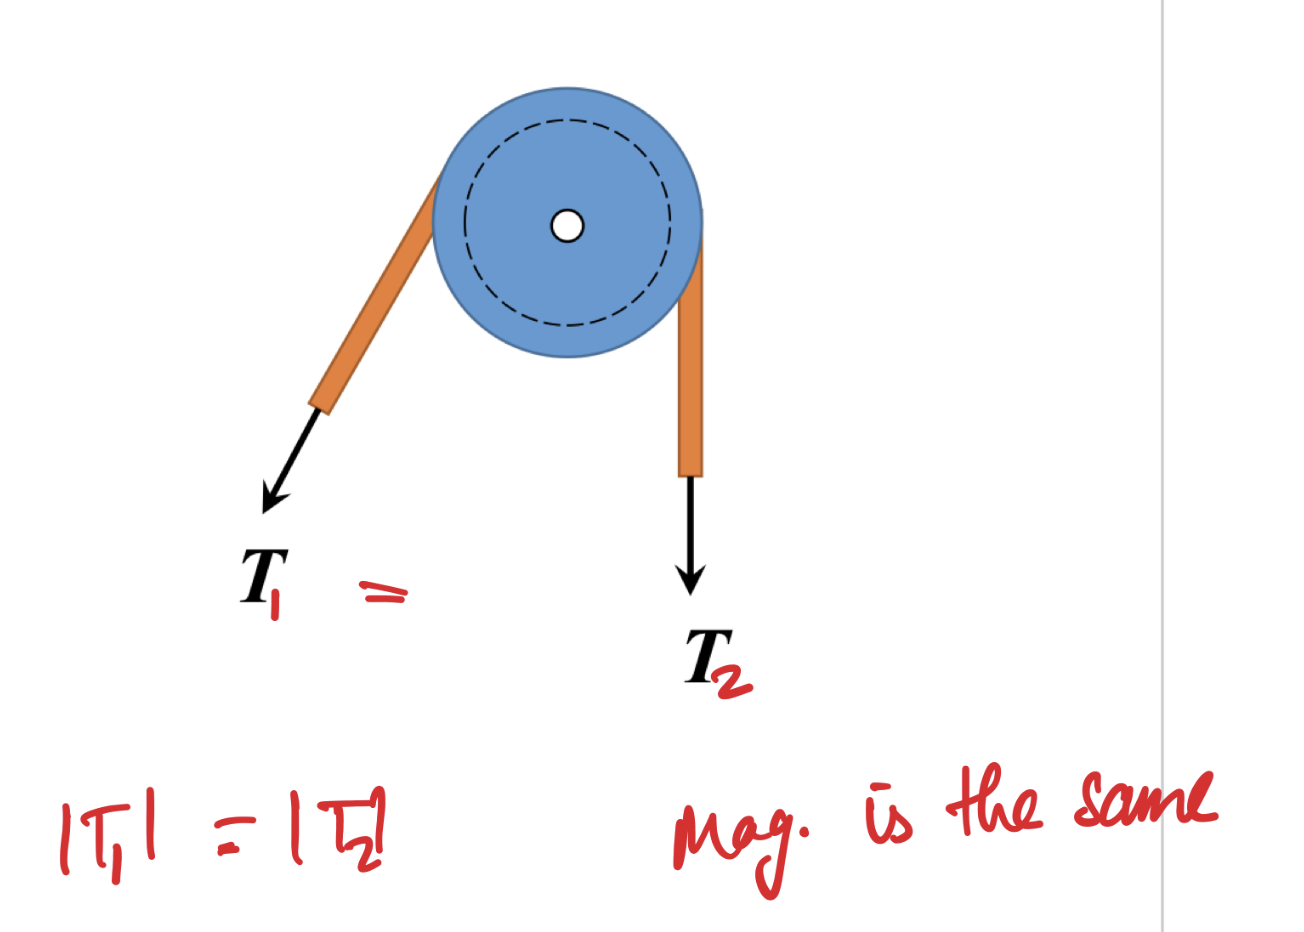
\includegraphics[angle=0, width=3in]{FBDFigures/PulleyAssumptions.png}
\vspace{-2mm}
\caption{\small \blue{Taken from TAM 210 Lecture 5 - Slide 6}}
\vspace{-3mm}
\label{Fig:PulleyAsusmptions}
\end{figure*}

\subsection{Spring Idealizations}

In this course, we assume springs are linearly elastic, which means that the force (tension) in the spring is linearly proportional to the extension of the spring ($s$) through the spring constant, $k$.

\[{F} = {k*s}\]

\[{s} = {l-l_0}\]

\begin{figure*}[!h]
\centering
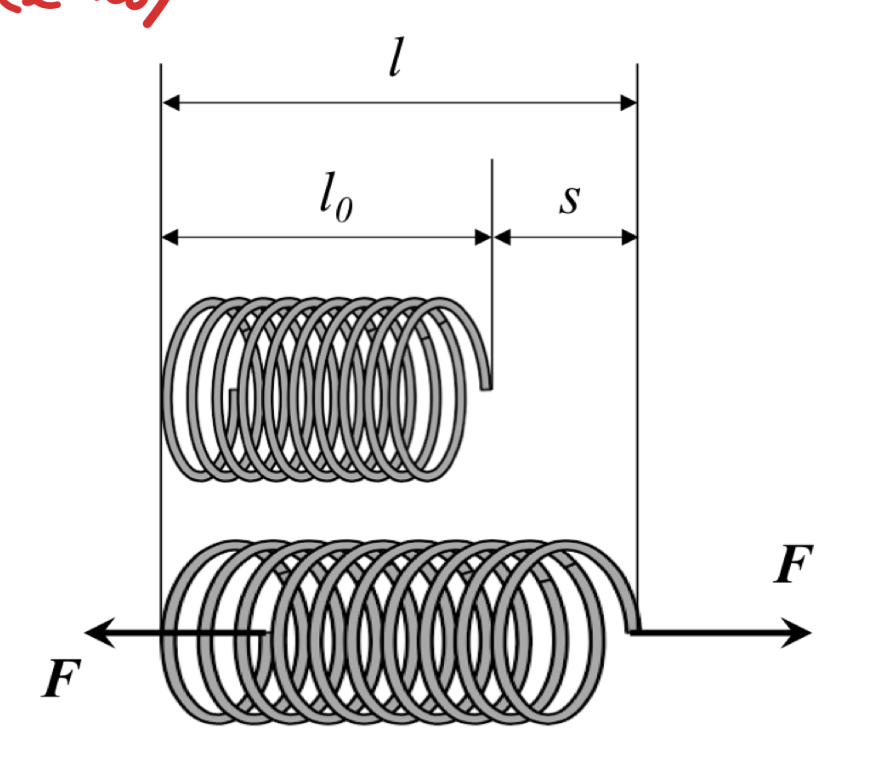
\includegraphics[angle=0, width=2in]{FBDFigures/SpringAssumptions.png}
\vspace{-2mm}
\caption{\small \blue{Taken from TAM 210 Lecture 5 - Slide 7. Make this picture and put it next to a stress-strain curve with the straight linear elastic line and the slope as k.}}
\vspace{-3mm}
\label{Fig:SpringAssumptions}
\end{figure*}

\subsection{Smooth Surface Idealizations}

If a surface is described as "smooth", we assume that there is no frictional force on the surface. Therefore, any force applied by the surface is normal to the surface. 

\begin{figure*}[!h]
\centering
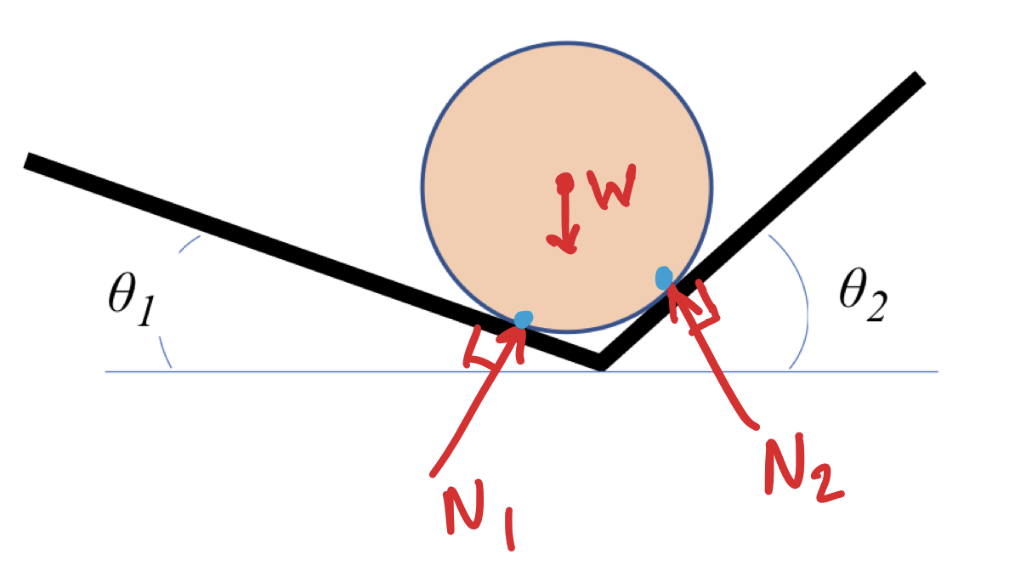
\includegraphics[angle=0, width=3in]{FBDFigures/SmoothAssumptions.png}
\vspace{-2mm}
\caption{\small \blue{Taken from TAM 210 Lecture 5 - Slide 8. This could become an interactive image eventually where the angles of the surfaces are changed by the user and then the reaction forces are also changing.}}
\vspace{-3mm}
\label{Fig:SmoothAssumptions}
\end{figure*}

%\subsection{\red{Equivalent force systems}}
%lecture 10
\section{Moments}

%Lectures 7, 8, 9, 10

A moment is a force applied at a distance from a point, which causes rotation about that point. 

The distance that the force is applied from is called the \textit{moment arm}. 

\begin{figure*}[!h]
\centering
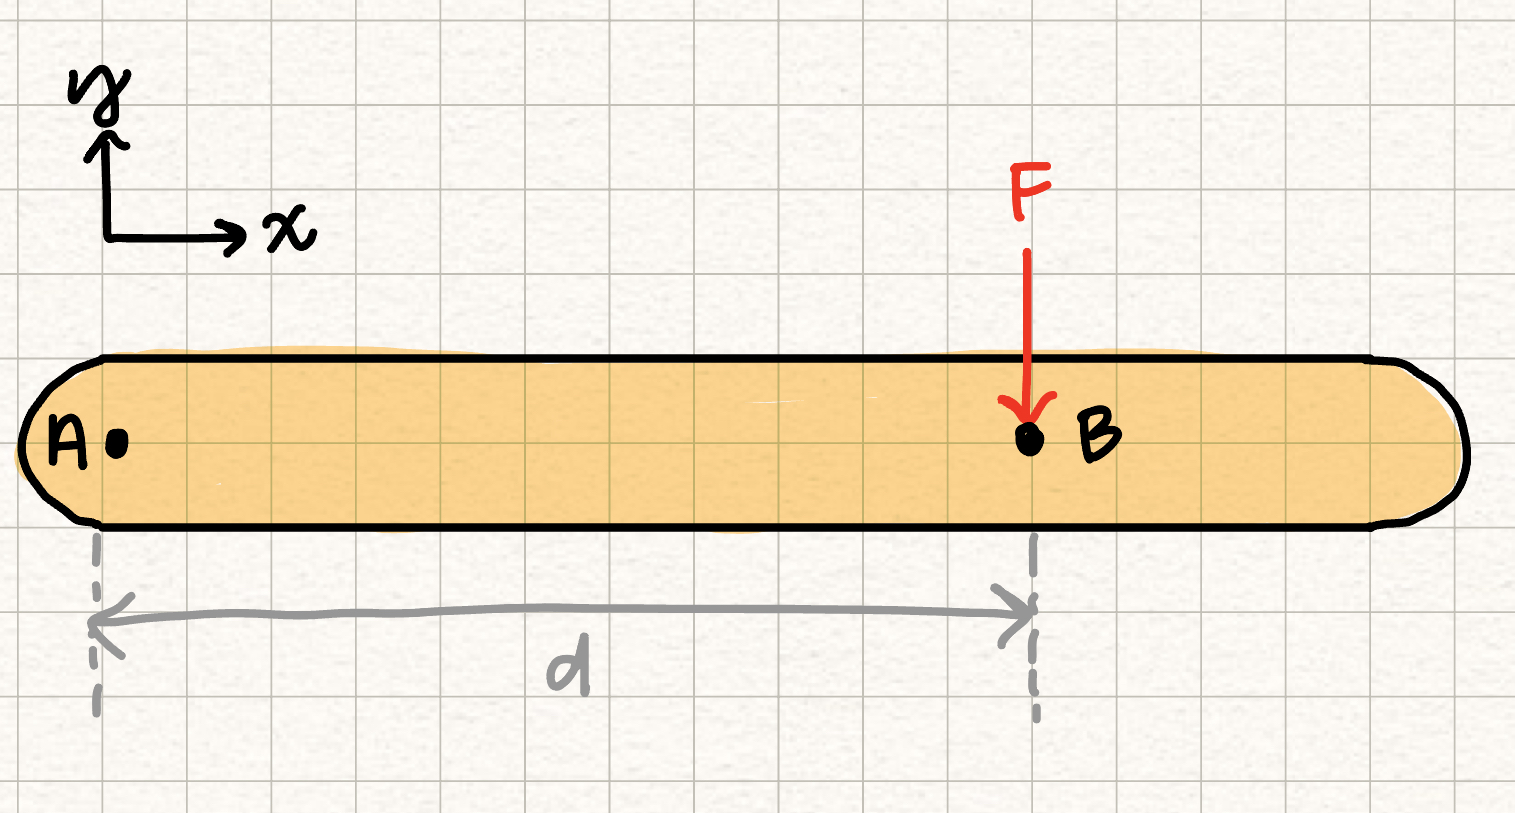
\includegraphics[angle=0, width=5in]{MomentsFigures/Moment.jpg}
\vspace{-2mm}
\caption{\small If the bar is pinned at point $A$, the force $F$, applied at a distance $d$ from point A, will cause a moment $M_A$ about point A and make the bar rotate clockwise.}
\vspace{-3mm}
\label{Fig:Moment}
\end{figure*}

The only force that produces a rotation about a point is a force perpendicular to the moment arm (in this case, the moment arm is $d$).

\blue{This could be a good place to add in example moments later in the side column for applications - could include muscle moments about a joint, oil rigs, the giant bucket that splashes water at a waterpark, pulling out a nail with a hammer.}

\subsection{Moments as scalars}

Moments can be written as scalar quantities, where 

\[{M_A} = F*d\]

Note that d is the distance from the applied force to the point of interest and that the force F is the force perpendicular to the moment arm. 

\begin{figure*}[!h]
\centering
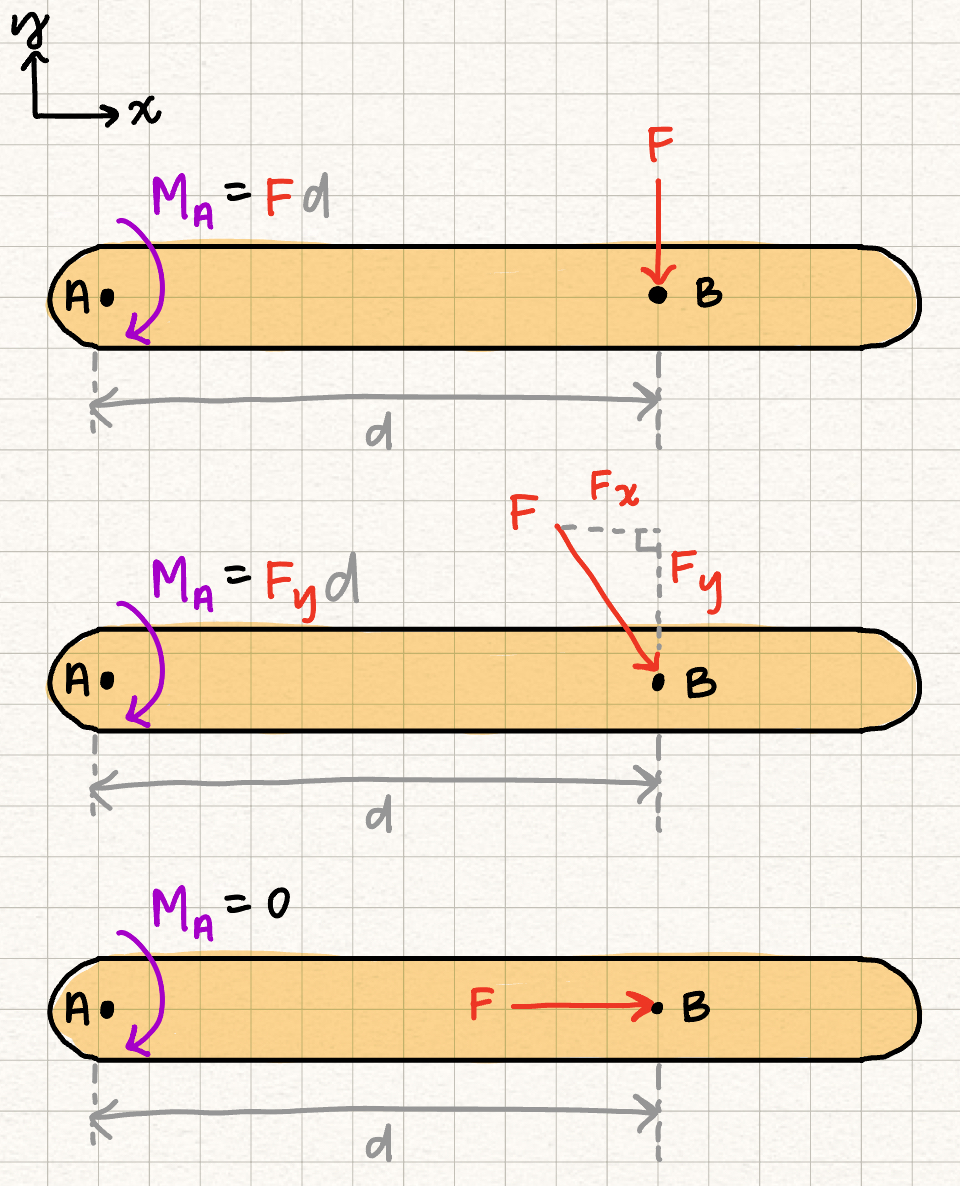
\includegraphics[angle=0, width=5in]{MomentsFigures/MomentScalar.jpg}
\vspace{-2mm}
\caption{\small The moment about point A is dependent on how much of the force $F$ is perpendicular to the moment arm $d$.}
\vspace{-3mm}
\label{Fig:MomentScalar}
\end{figure*}



You can determine the direction of moments using the right hand rule and wrapping your fingers around where the moment is turning. The direction your thumb is pointing is the direction of the moment. 

Moments are assumed to be positive when they point in the $-\hat{k}$ direction (clockwise rotation) and negative when they point in the $+\hat{k}$ direction (counterclockwise rotation). 

\begin{figure*}[!h]
\centering
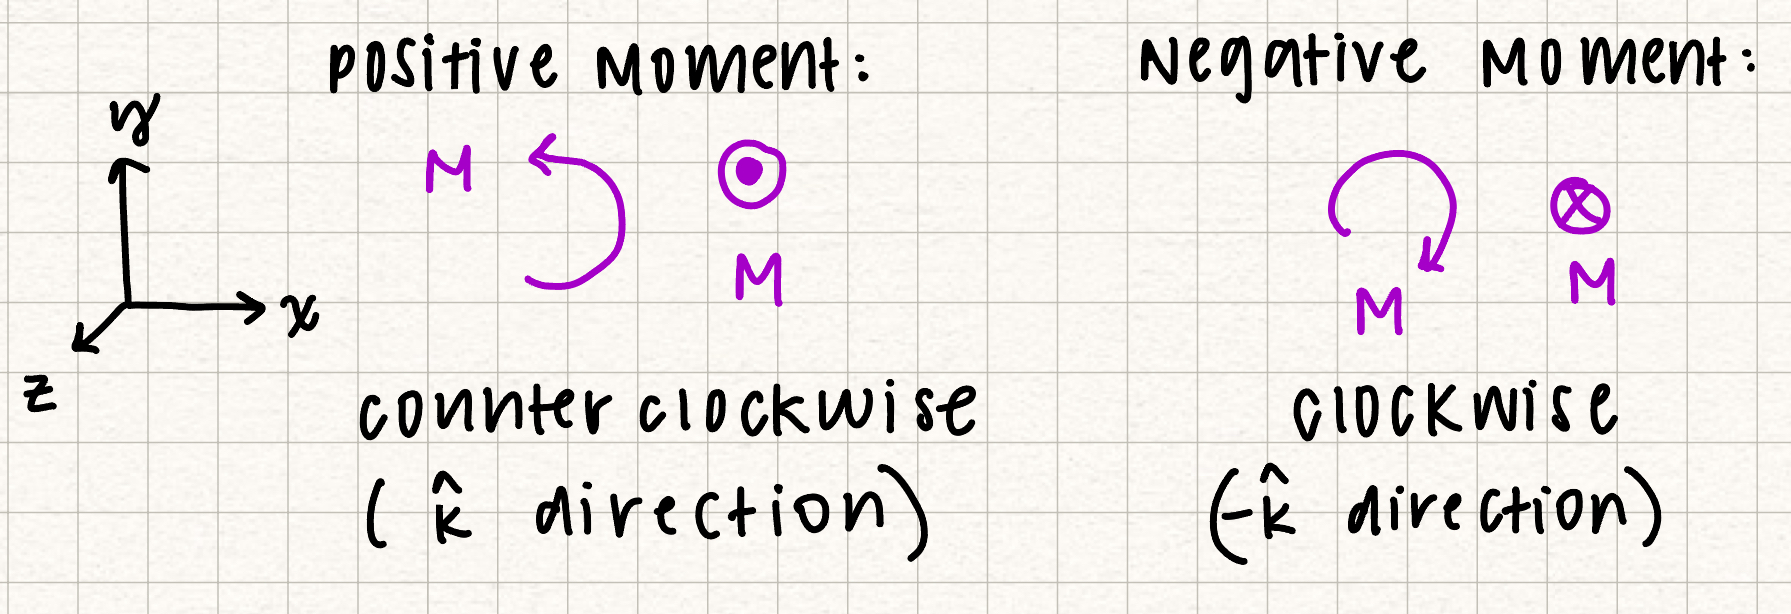
\includegraphics[angle=0, width=5in]{MomentsFigures/MomentConventions.jpg}
\vspace{-2mm}
\caption{\small Positive and negative moment conventions.}
\vspace{-3mm}
\label{Fig:MomentConventions}
\end{figure*}

%lectures 7 and 8

\subsection{Moments as vectors}

Moments can also be written as vector quantities, where the moment about point A is the cross product of the moment arm, $r$ and the force $F$. 

\[\vec{M_A} = \vec{r} \times \vec{F}\]

Using this formula, moments could have an $\hat{i}$, $\hat{j}$, and $\hat{k}$ component. 

The magnitude of the moment can be written as 

\[\vert\vec{M_A}\vert = \vert\vec{r}\vert \vert\vec{F}\vert sin\theta\]

%lectures 7 and 8

\subsection{\red{Couple Moment}}

A couple moment is a set of two equal and opposite forces with parallel lines of action that produce a moment. 

The resulting moment from a force couple can be written as 

\[M_A = F*d_{\perp}\]

where $F$ is the magnitude of one of the force vectors and d is the perpendicular distance between the two vectors. 

Note: Couple moments are independent of location when applied to a rigid body, which means the resulting moment from a force couple can be "placed" anywhere on the rigid body with the same resulting rotation from the couple moment. 

\begin{figure*}[!h]
\centering
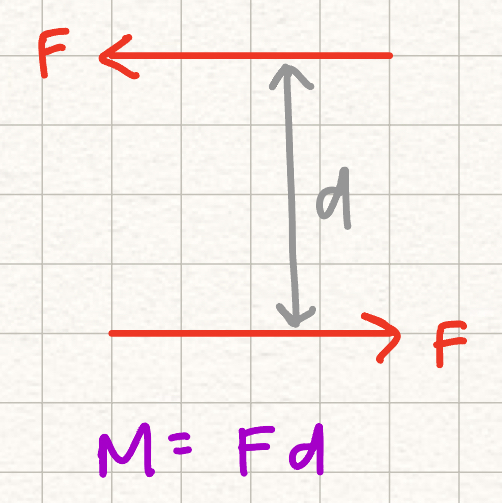
\includegraphics[angle=0, width = 2.5in]{MomentsFigures/CoupleMoment.jpg}
\vspace{-2mm}
\caption{\small A couple moment}
\vspace{-3mm}
\label{Fig:CoupleMoment}
\end{figure*}

%In vector notation, a couple moment can be written as 

%lectures 9 and 10

%\subsection{\red{Moment about an axis}}

%\red{Not sure that this needs to be a section }
\section{Force Systems}

\subsection{Equivalent systems}

\blue{Do we need this section?}

It can be helpful at times to reduce the forces on a body and combine resultant moments and simplify the analysis. For example, you can replace a force couple with their equivalent couple moment in a system. 

These forces and moments will have the same external effect on the body, but the internal forces on the rigid body may be different. 

\subsection{Concentrated forces}

\blue{Do we need this section? - from lecture 2}

Concentrated forces are forces acting at a specific point on a body. 

\begin{figure*}[!h]
\centering
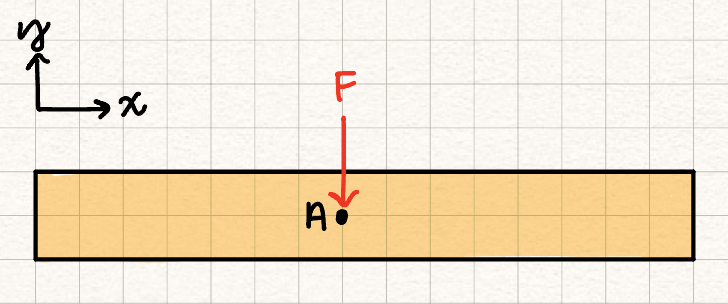
\includegraphics[angle=0, width=5 in]{ForceSystemsFigures/ConcentratedForce.PNG}
\vspace{-2mm}
\caption{\small A concentrated force applied to a bar at point A.}
\vspace{-3mm}
\label{Fig:ConcLoad}
\end{figure*}

\subsection{Distributed loads}
%from lecture 11 and 12

Distributed loads (usually written as $w(x)$) are forces applied over a length, volume, or area. The SI units for distributed loads are N/m. These loads, written as a function of length $x$ can be simplified into an equivalent force, $F_R$, which results in the same external loading on the rigid body. 

The magnitude of the equivalent force $F_R$ is the area under the $w(x)$ curve. The location of the resultant force $F_R$ is the location of the centroid of the shape of the force curve. 

\blue{Later, we can add a side comment about examples of distributed loads in real life. For example, books on a bookshelf, air pressure over a lake, the distribution of loads on on the ground over your foot when you take a step}

\subsubsection{Rectangular loading}

For a constant distributed load of magnitude c applied to a bar over a length l, the resultant force magnitude is 

\[F_R = c*l\]

the resultant force location is at $l/2$.

\begin{figure*}[!h]
\centering
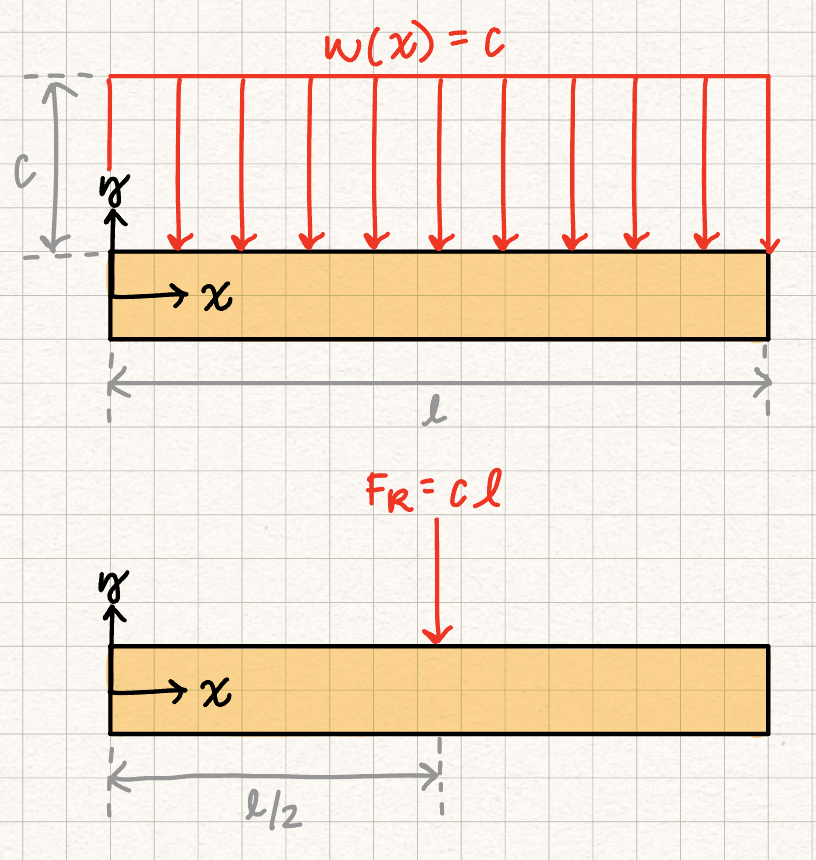
\includegraphics[angle=0, width=5 in]{ForceSystemsFigures/DistLoad.PNG}
\vspace{-2mm}
\caption{\small Example distributed load (top) and its equivalent force system (bottom).}
\vspace{-3mm}
\label{Fig:DistLoad}
\end{figure*}


\subsubsection{Triangular loading}

For a triangular distributed load (a uniformly varying load), the magnitude of the load is equivalent to the area of the triangle. 

\[F_R = 0.5*c*l\]

The location of $F_R$ is 1/3 from the base of the triangle. 


\begin{figure*}[!h]
\centering
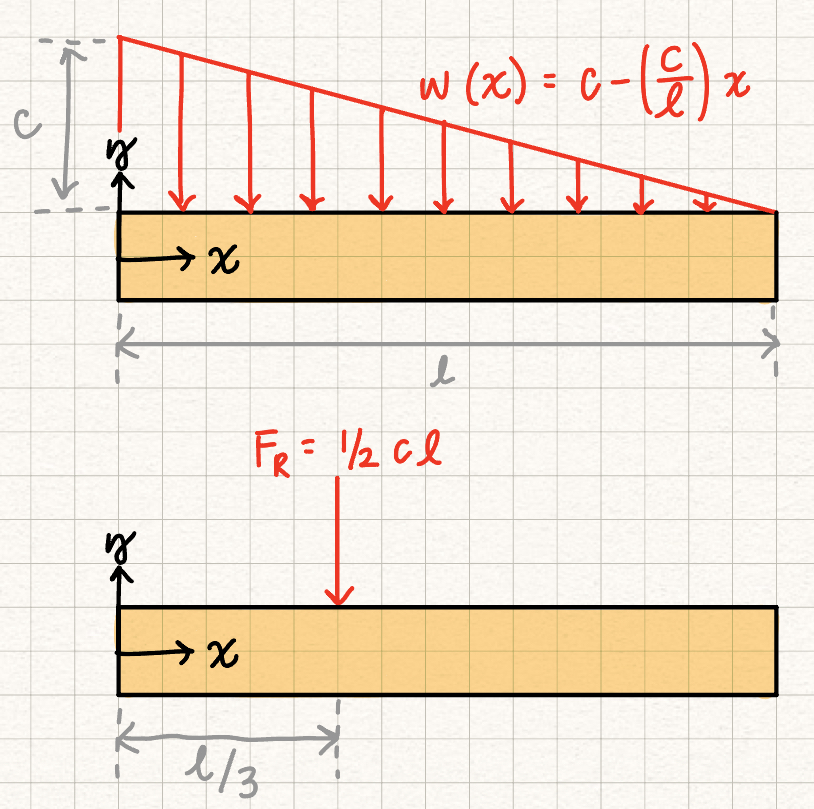
\includegraphics[angle=0, width=5 in]{ForceSystemsFigures/TriangleLoad.PNG}
\vspace{-2mm}
\caption{\small Example triangular distributed load (top) and its equivalent force system (bottom).}
\vspace{-3mm}
\label{Fig:TriLoad}
\end{figure*}

%from lecture 11 and 12

\subsubsection{Nonuniform distributed loads}

More complex distributed loads can be reduced to two distributed loads of uniform shape, or the integral of the distributed load function can be taken to obtain the area under $w(x)$, which is $F_R$. 

\[F_R = \int_{0}^{L} w(x) \,dx \]

The location of $F_R$ on the beam can be found by solving for the moment $M_R$ about a point. In this case we will take the moment about the point $x$=0 and setting it equivalent to the moment produced by the resultant force $F_R$ at $x$=0. 

\[M_R = \int_{0}^{L} x*w(x) \,dx = \bar{x}*F_R\]

Now we can solve for the center of mass of the distributed load, $\bar{x}$, using

\[\bar{x} = \dfrac{M_R}{F_R}\]

\begin{figure*}[!h]
\centering
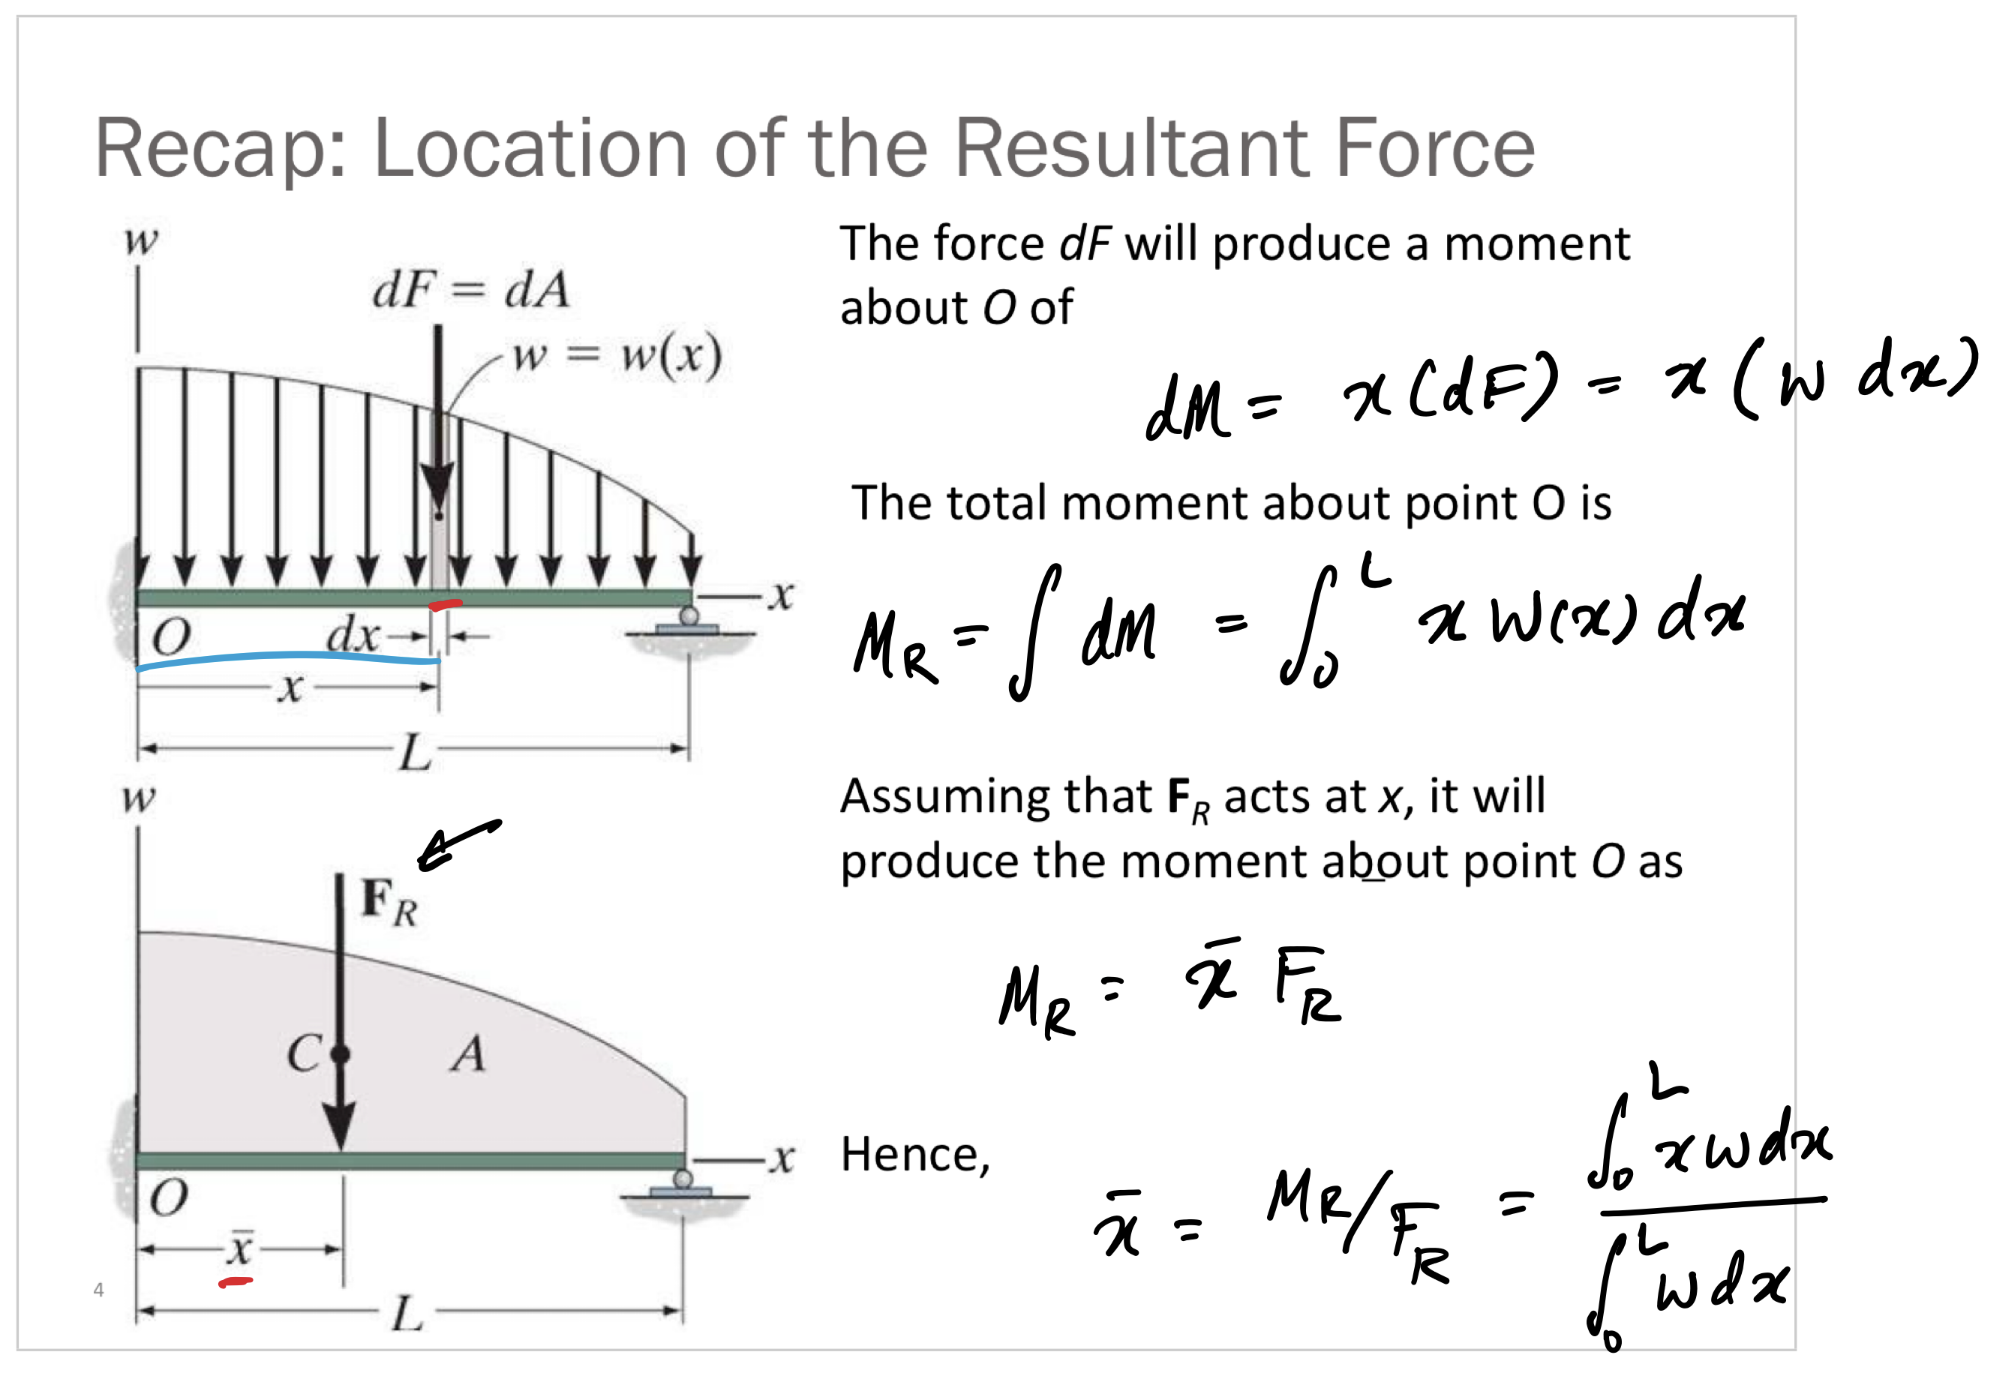
\includegraphics[angle=0, width=5 in]{ForceSystemsFigures/NonuniformLoad.PNG}
\vspace{-2mm}
\caption{\small Nonuniform load. Need to remake this in the same style as the other pictures.}
\vspace{-3mm}
\label{Fig:NonUniLoad}
\end{figure*}


%from lecture 11 and 12
\section{Reaction Forces}

\subsection{Types of Connections}

\begin{figure*}[!h]
\centering
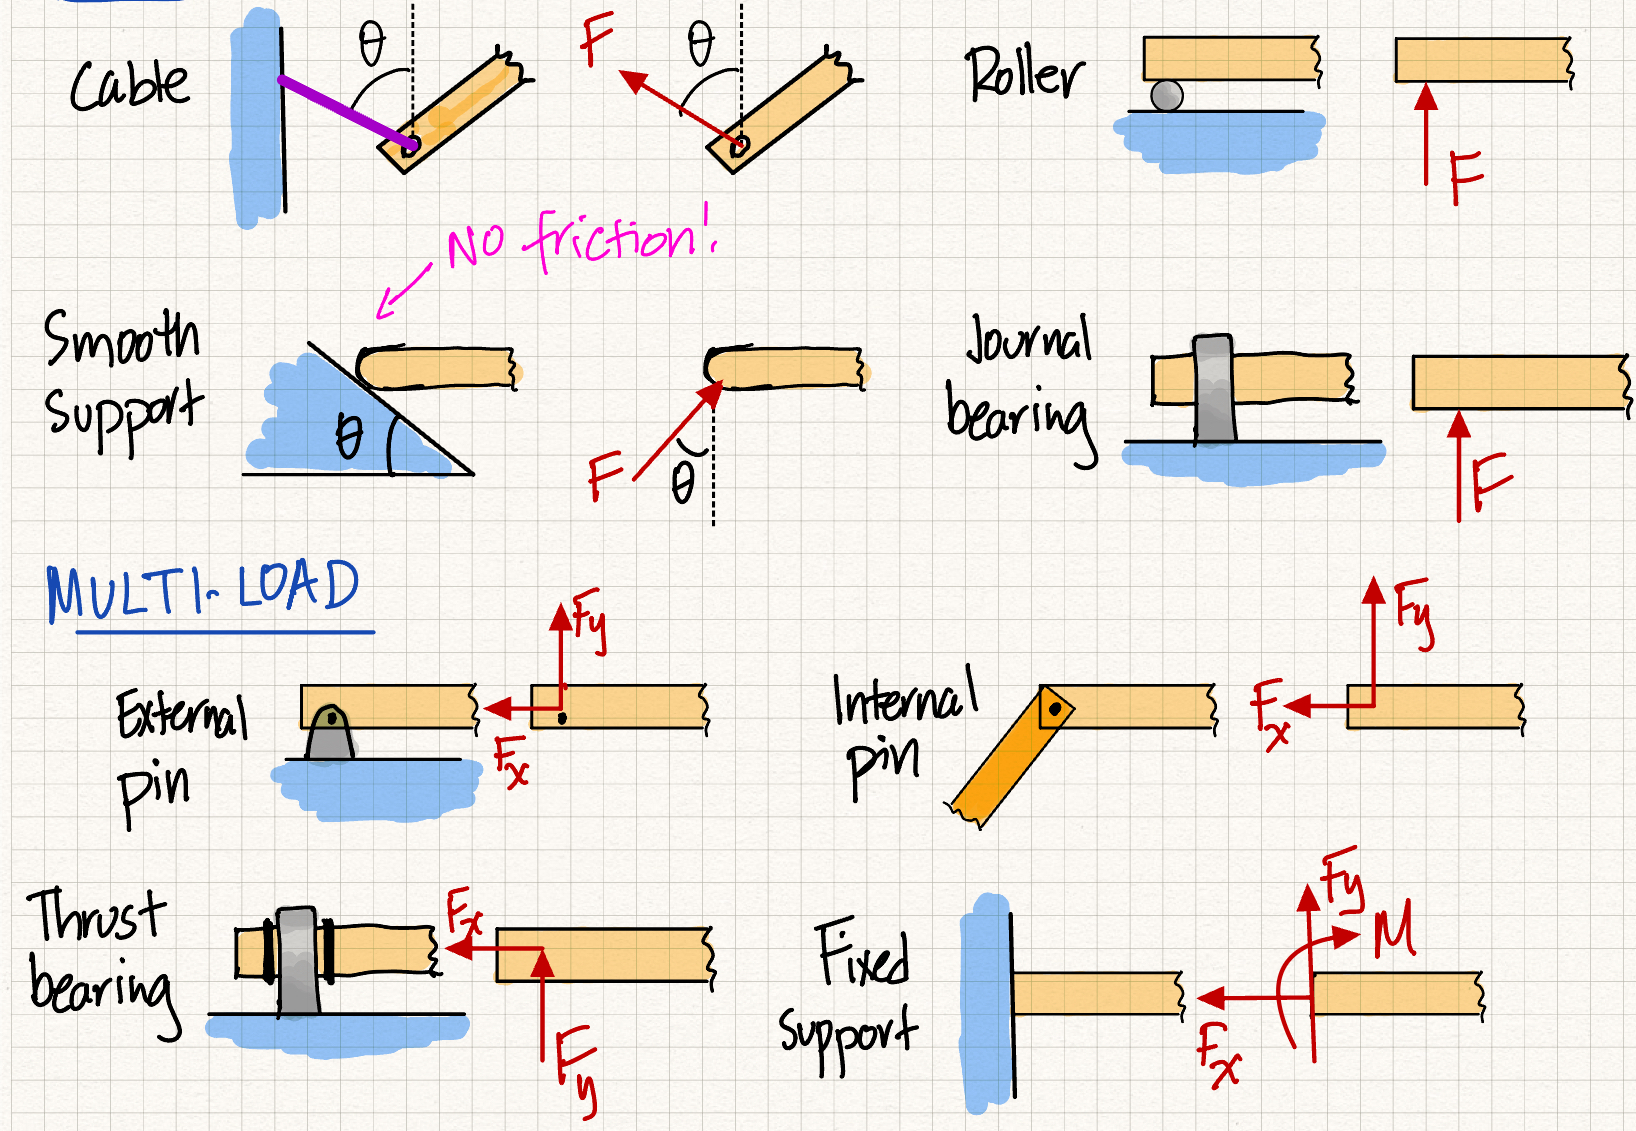
\includegraphics[angle=0, width=\textwidth]{ReactionForcesFigures/ReactionForces.jpg}
\vspace{-2mm}
\caption{\small \blue{Taken from Mariana Kersh's TAM 251 Lecture notes}}
\vspace{-3mm}
\label{Fig:NewtonsLaws}
\end{figure*}

\blue{Should we make a table for here? Some good examples of rigid constraints in real life in lecture 15.}

%From lecture 13

\blue{L13, Slide 3 had some good examples of support reactions if we want to make a pop up on the side eventually.}

\subsection{Redundant Constraints}

If a body has more supports than it needs to hold it in equilibrium, it is overly constrained. This will result in more unknown reaction forces than equations we can write, and the problem will not be solvable using statics alone. This type of system is a "statically indeterminate" system. 

%From lecture 15
\section{Internal Forces}

Internal forces of a member can be determined by creating an imaginary cut in a member, and then solving for the internal shear force, normal force, and bending moment (which, after the cut, become "external" forces that can be solved for). 

To determine how the internal shear force and bending moment change throughout the member, shear force and bending moment diagrams are created. Shear force diagrams provide a graphical representation of the internal shear force within a member, and bending moment diagrams provide a graphical representation of the internal bending moment within a member. 

\begin{figure*}[!h]
\centering
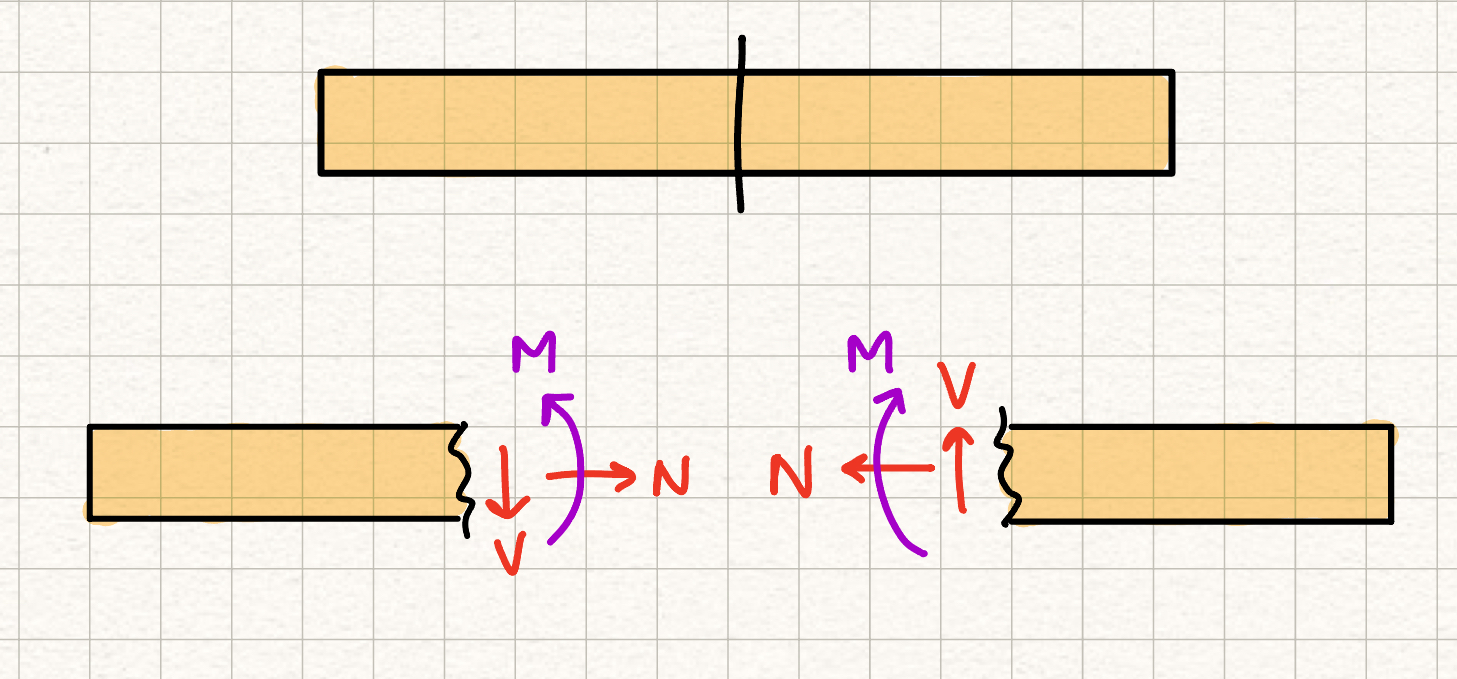
\includegraphics[angle=0, width=5 in]{IntForceFigures/IntForces.jpg}
\vspace{-2mm}
\caption{\small Internal shear force (V), internal normal force (N), and internal moment (M).}
\vspace{-3mm}
\label{Fig:IntForces}
\end{figure*}

%starts in lecture 19

\subsection{Sign Conventions}

\begin{figure*}[!h]
\centering
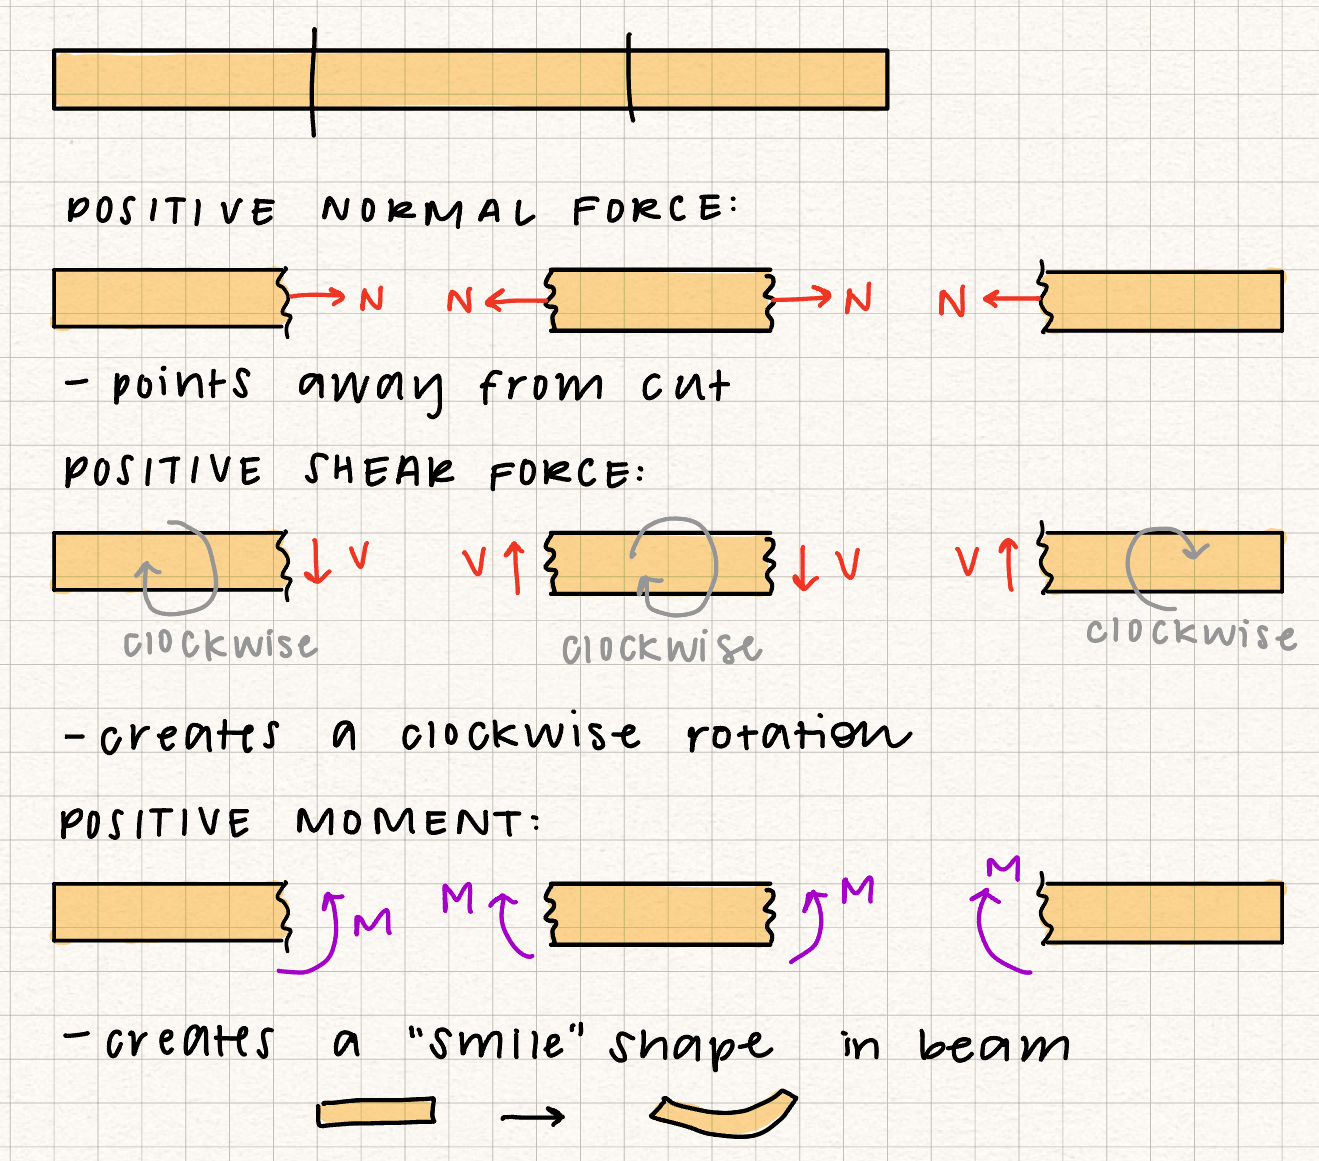
\includegraphics[angle=0, width=\textwidth]{IntForceFigures/SignConventions.jpg}
\vspace{-2mm}
\caption{\small Sign conventions for internal forces and moments}
\vspace{-3mm}
\label{Fig:SignConventions}
\end{figure*}


\subsection{General Procedure}

Creating a shear force and bending moment diagram allows us to create a graphical representation of $V$ and $M$ as a function of the position along the beam, $x$. Therefore when creating internal loading diagrams we are trying to write equations for $V(x)$ and $M(x)$.

\begin{figure*}[!h]
\centering
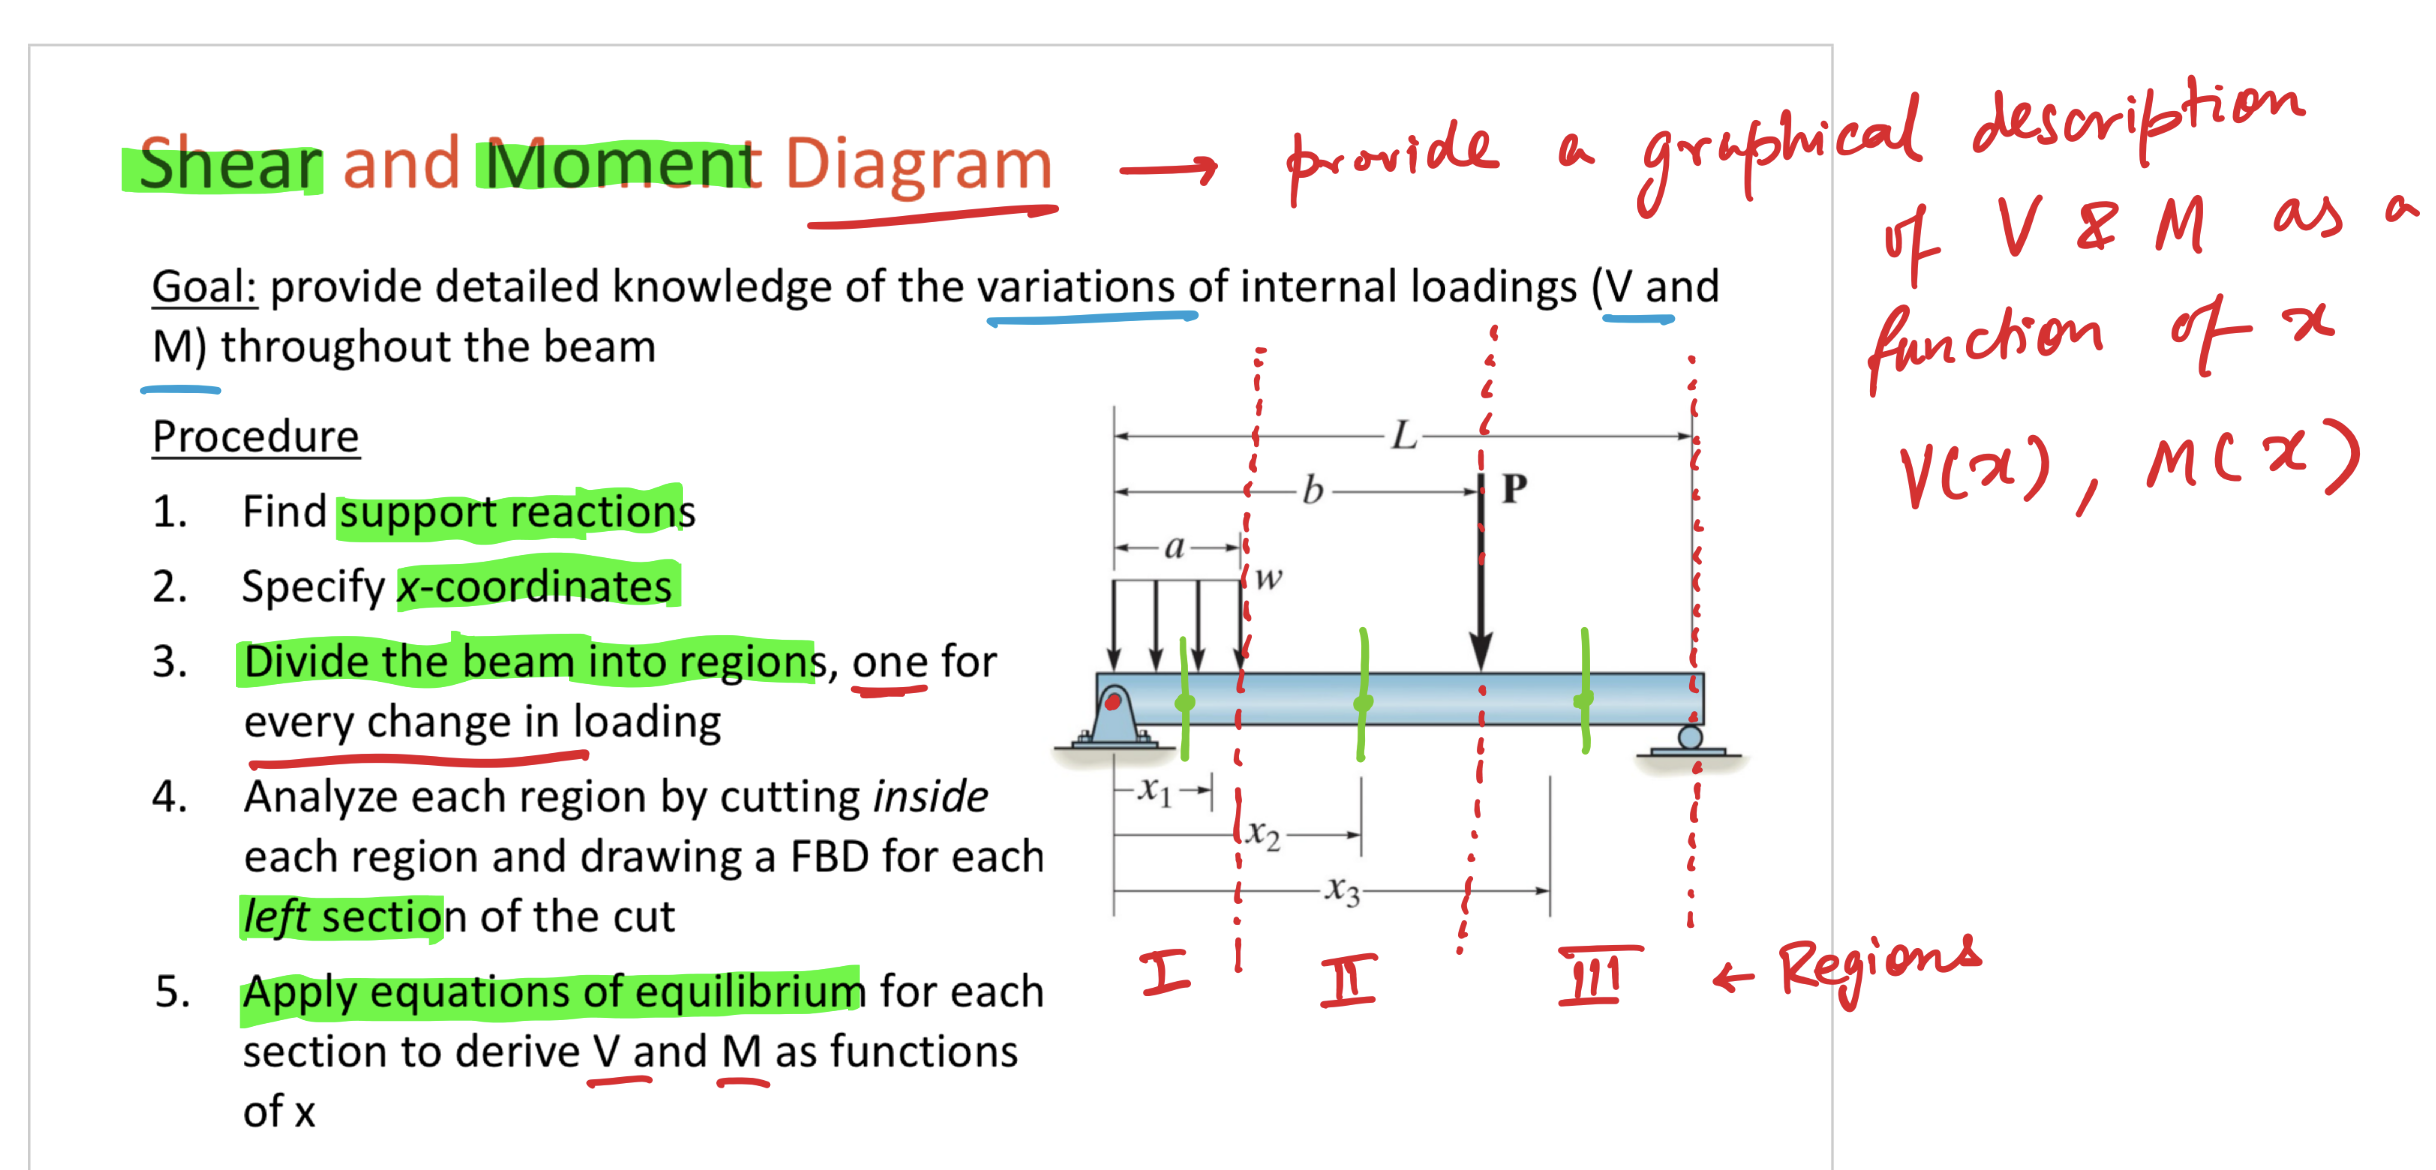
\includegraphics[angle=0, width=\textwidth]{IntForceFigures/DiagramProcedure.png}
\vspace{-2mm}
\caption{\small \blue{Taken from TAM 210 Lecture 22}}
\vspace{-3mm}
\label{Fig:DiagramProcedure}
\end{figure*}

\begin{figure*}[!h]
\centering
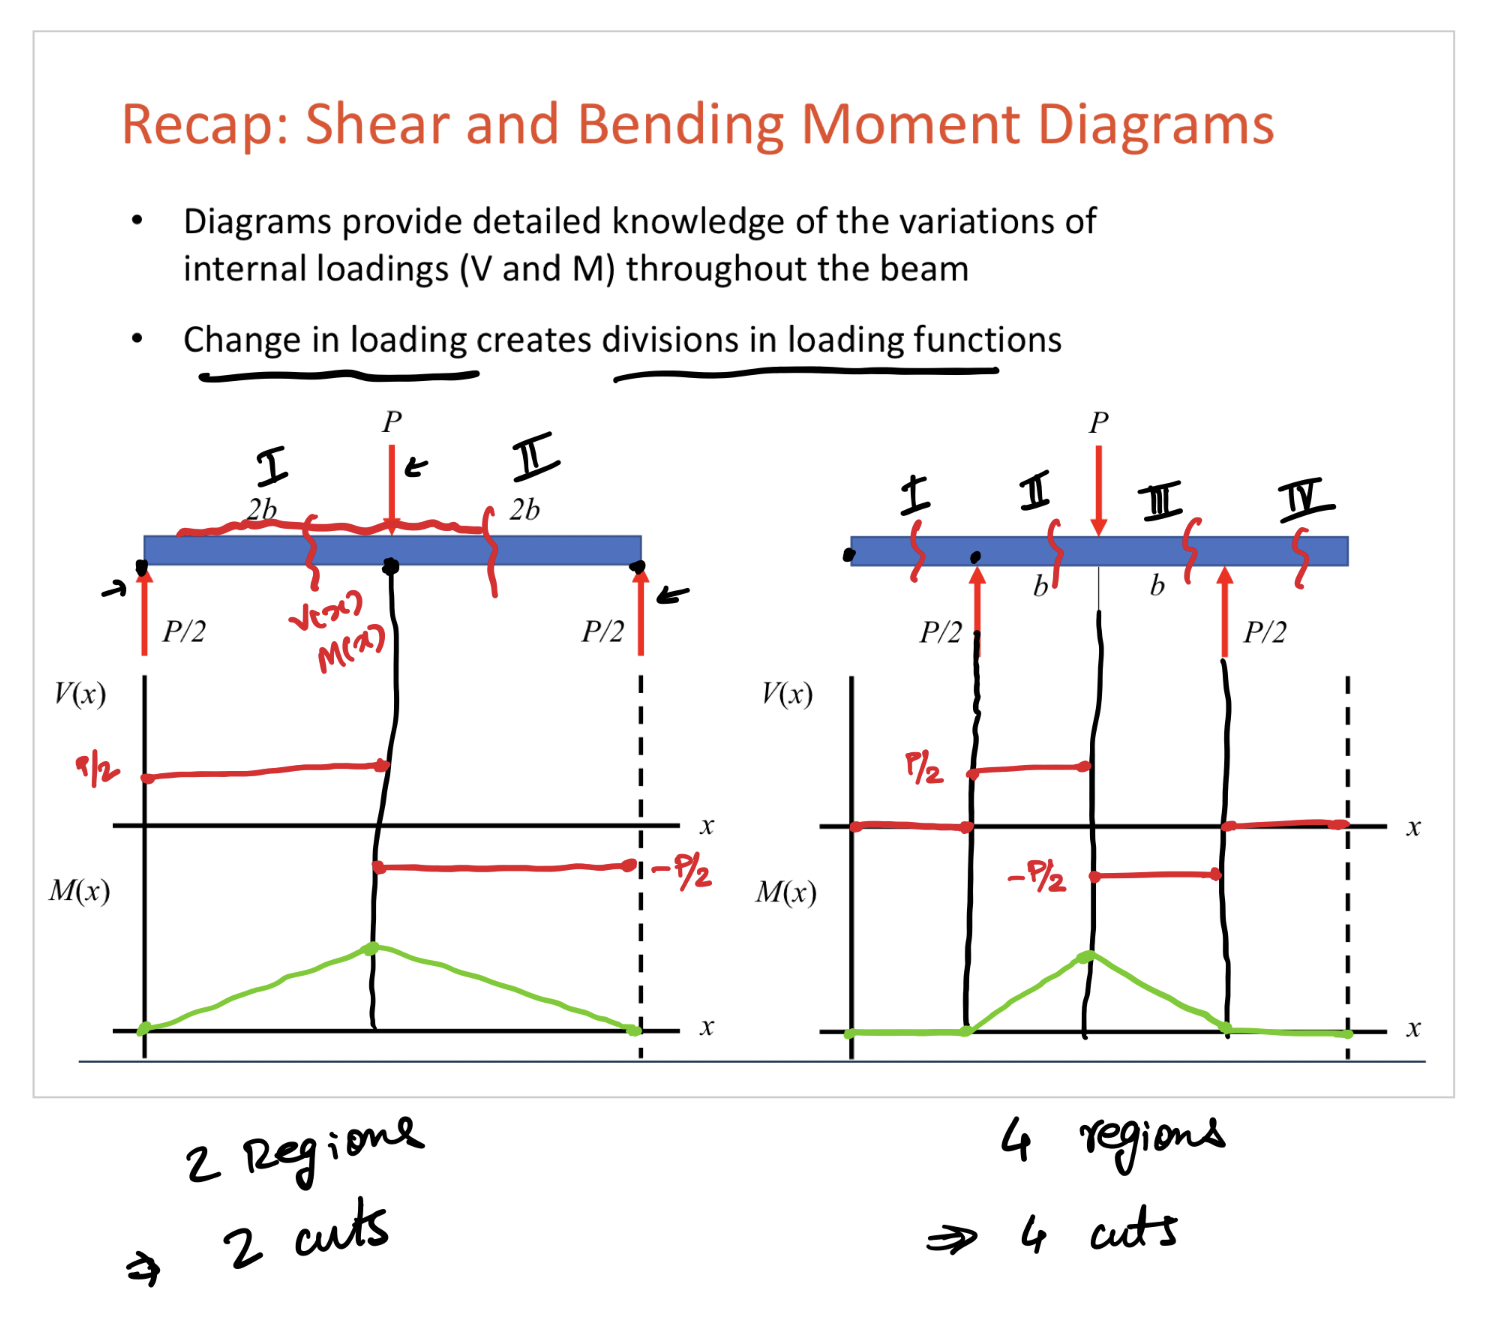
\includegraphics[angle=0, width=\textwidth]{IntForceFigures/IntLoadRecap.png}
\vspace{-2mm}
\caption{\small \blue{Taken from TAM 210 Lecture 23}}
\vspace{-3mm}
\label{Fig:DiagramProcedure}
\end{figure*}

\subsection{\red{General Rules}}

\begin{enumerate}
    \item When there is an external concentrated force or moment, there will be a "jump" in the shear force or bending moment diagram
    \item $w(x)$, $V$, and $M$ are related via the following relationship: 
\end{enumerate}

\begin{figure*}[!h]
\centering
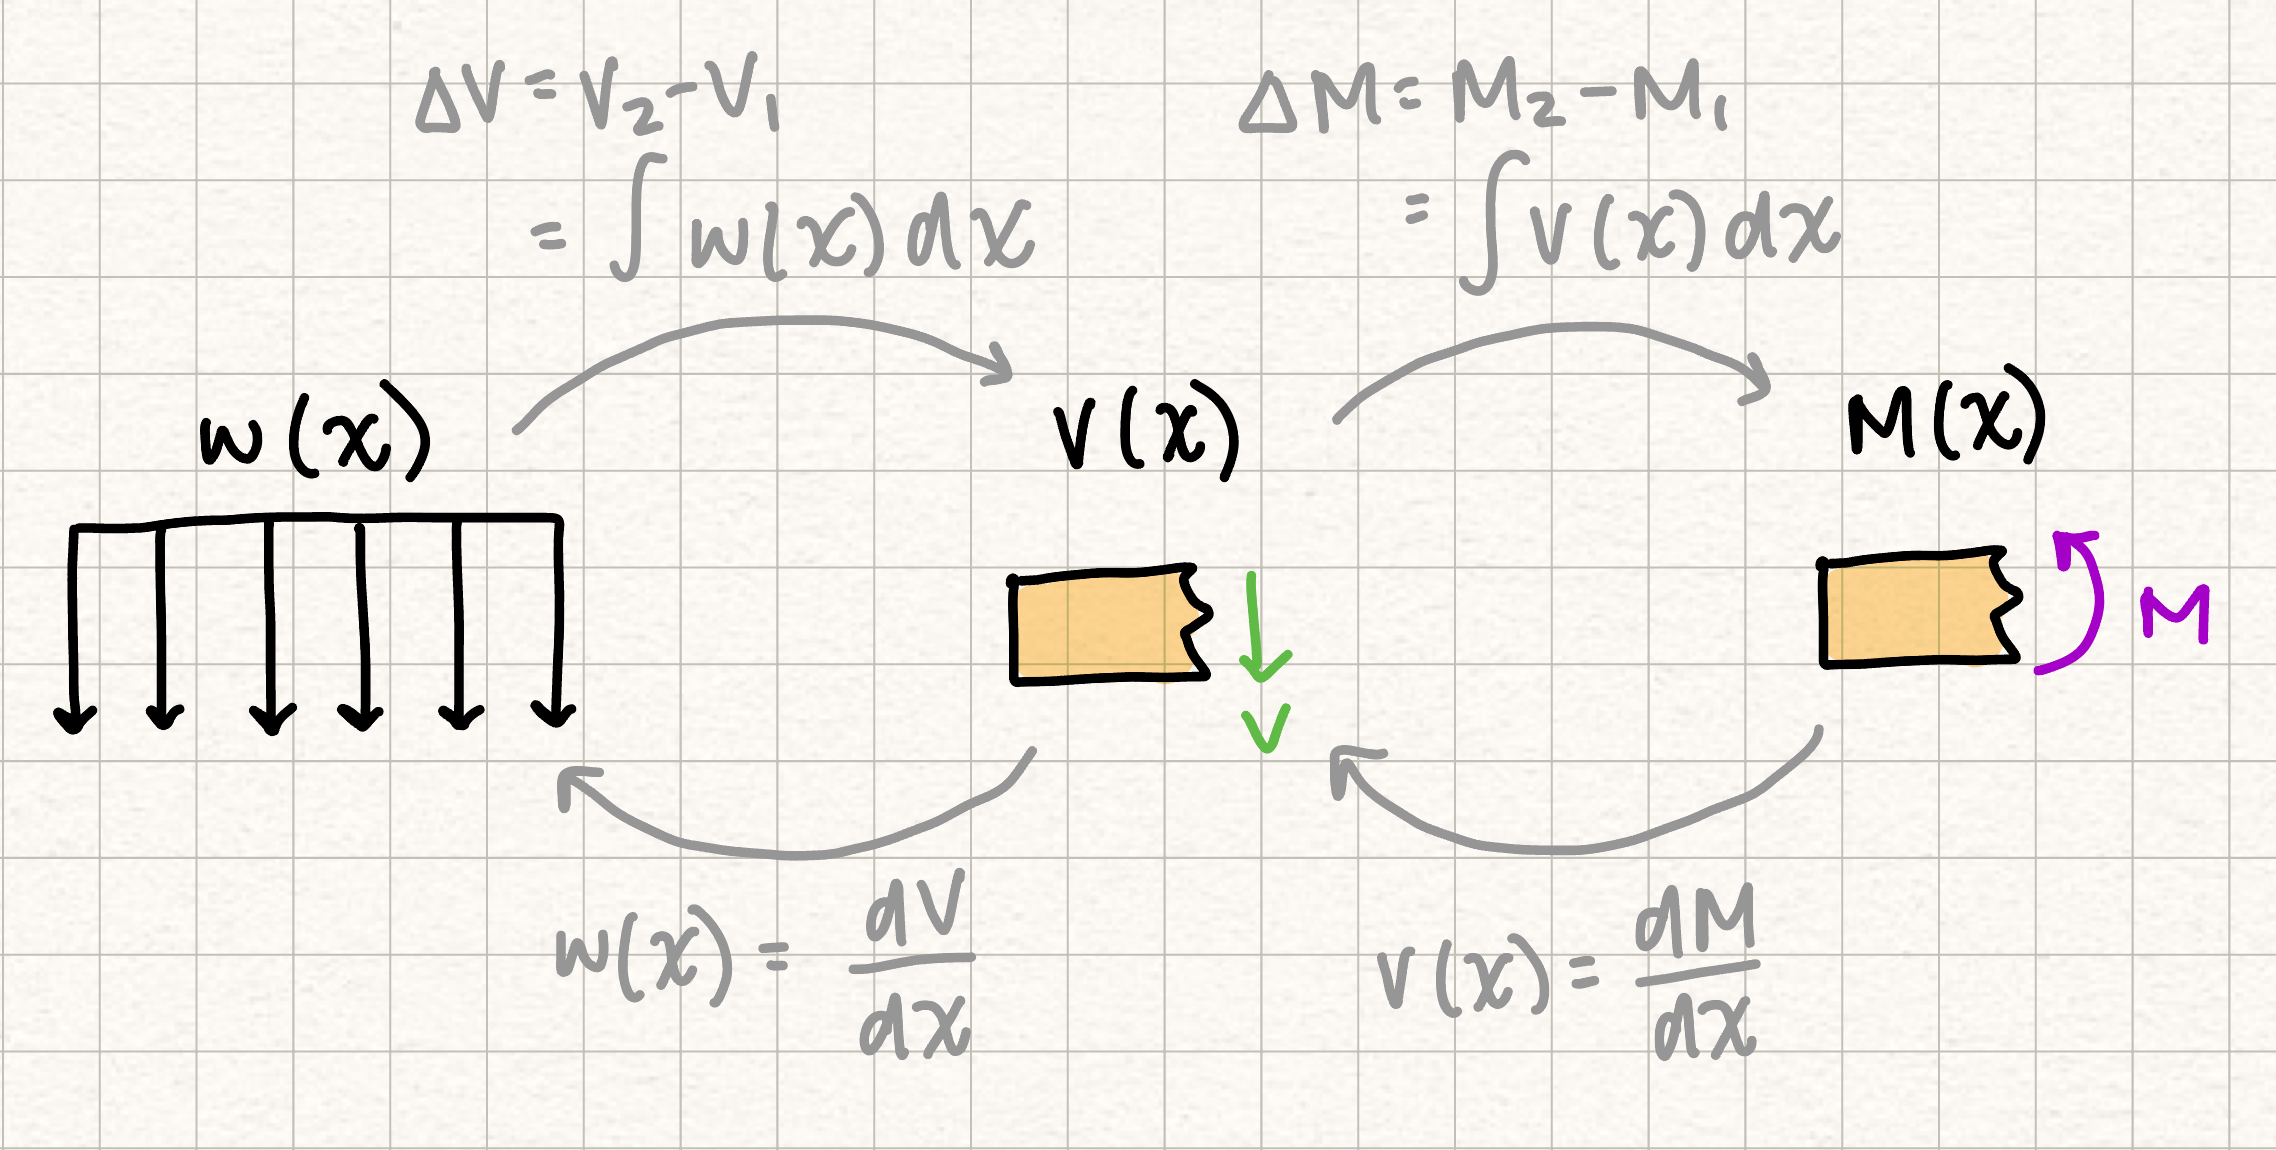
\includegraphics[angle=0, width=\textwidth]{IntForceFigures/IntDerivRelationships.jpg}
\vspace{-2mm}
\caption{\small \blue{See TAM 210 Lecture 25}}
\vspace{-3mm}
\label{Fig:IntForceRelationships}
\end{figure*}

\subsection{\red{Shear Force Diagram}}

%Lecture 22, 23, 24

\subsection{\red{Bending Moment Diagram}}

%Lecture 22, 23, 24

\section{Trusses}

Trusses are support members that are joined together at the ends. The function of a truss is to transmit loads to a support joint. In this section, we will analyze a simplified version of planar trusses called simple trusses, which consist of two-force members connected by frictionless joints/pins.

%starting in lecture 16

%Definition of a truss

\subsection{Truss Assumptions}

The main assumptions for trusses and truss structures are:

\begin{enumerate}
    \item {All loading is applied at the joints.}
    \item{The weight of the truss is negligible.}
\end{enumerate}

Because of these assumptions, all trusses are \textit{two force members}, with the forces on the truss acting along the axis of the member. 
%good summary in lecture 17, slide 5

\subsection{Two Force Member}

A two force member is a rigid body that has two forces (no moments) acting on it in two locations. 

Assumptions of two force members (for equilibrium to hold): 
\begin{enumerate}
\item{$|F_A| = |F_B|$}
\item{$\vec{F_A} + \vec{F_B} = 0$}
\item{$\vec{F_A}$ and $\vec{F_B}$ act along the same line of action.}
\end{enumerate}

\begin{figure*}[!h]
\centering
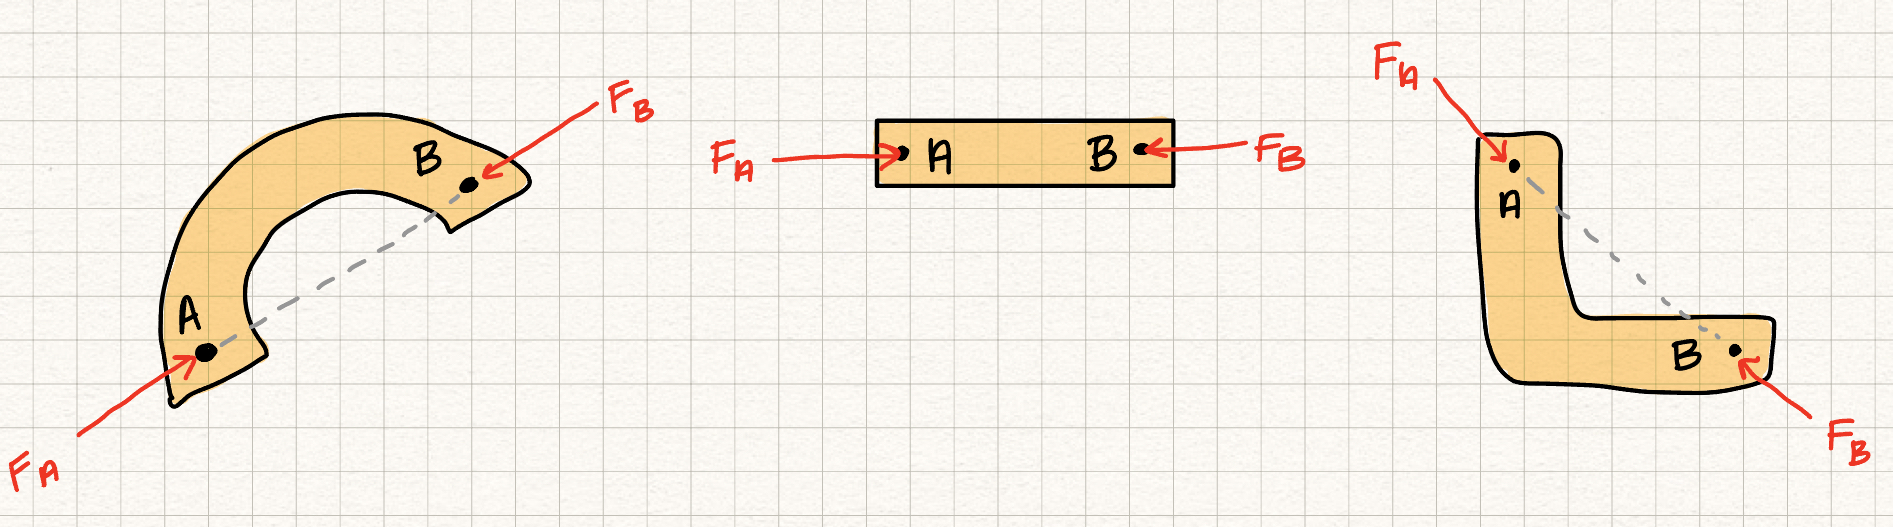
\includegraphics[angle=0, width=5in]{TrussFigures/2ForceMembers.jpg}
\vspace{-2mm}
\caption{\small Examples of different two force members.}
\vspace{-3mm}
\label{Fig:2ForceMembers}
\end{figure*}

    
%Lecture 16
\subsection{Zero Force Member}

Zero force members are members in a truss structure that experience no force. They act as support trusses to add stability, but are not load bearing. There are 2 cases where zero force members occur: 
\begin{enumerate}
    \item Two noncolinear members share a pin with no support or external forces (Zero force member example, left)
    \item Two colinear forces with a third noncolinear force on a pin (zero force member example, right)
\end{enumerate}

\begin{figure*}[!h]
\centering
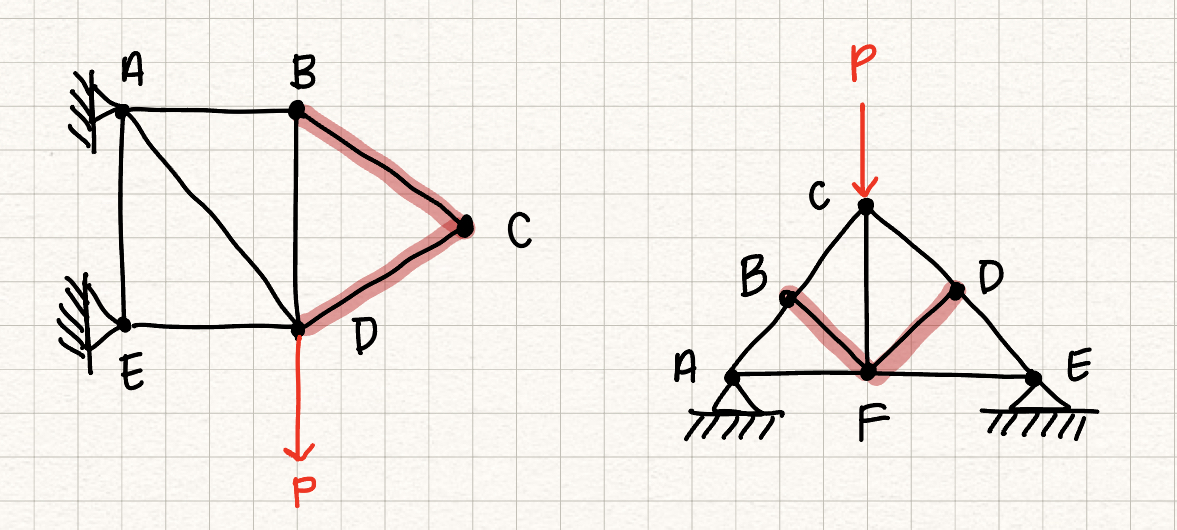
\includegraphics[angle=0, width=5in]{TrussFigures/0ForceMembers.jpg}
\vspace{-2mm}
\caption{\small Examples of different zero force members, highlighted in red.}
\vspace{-3mm}
\label{Fig:0ForceMembers}
\end{figure*}

\blue{Insert content here from TAM 212 reference page - Free Body Diagrams - Rigid Bodies - Trusses section. This has a really good analysis of eliminating zero force members to simplify the structure}

%lecture 18

\subsection{Truss Analysis: Joints}

\begin{figure*}[!h]
\centering
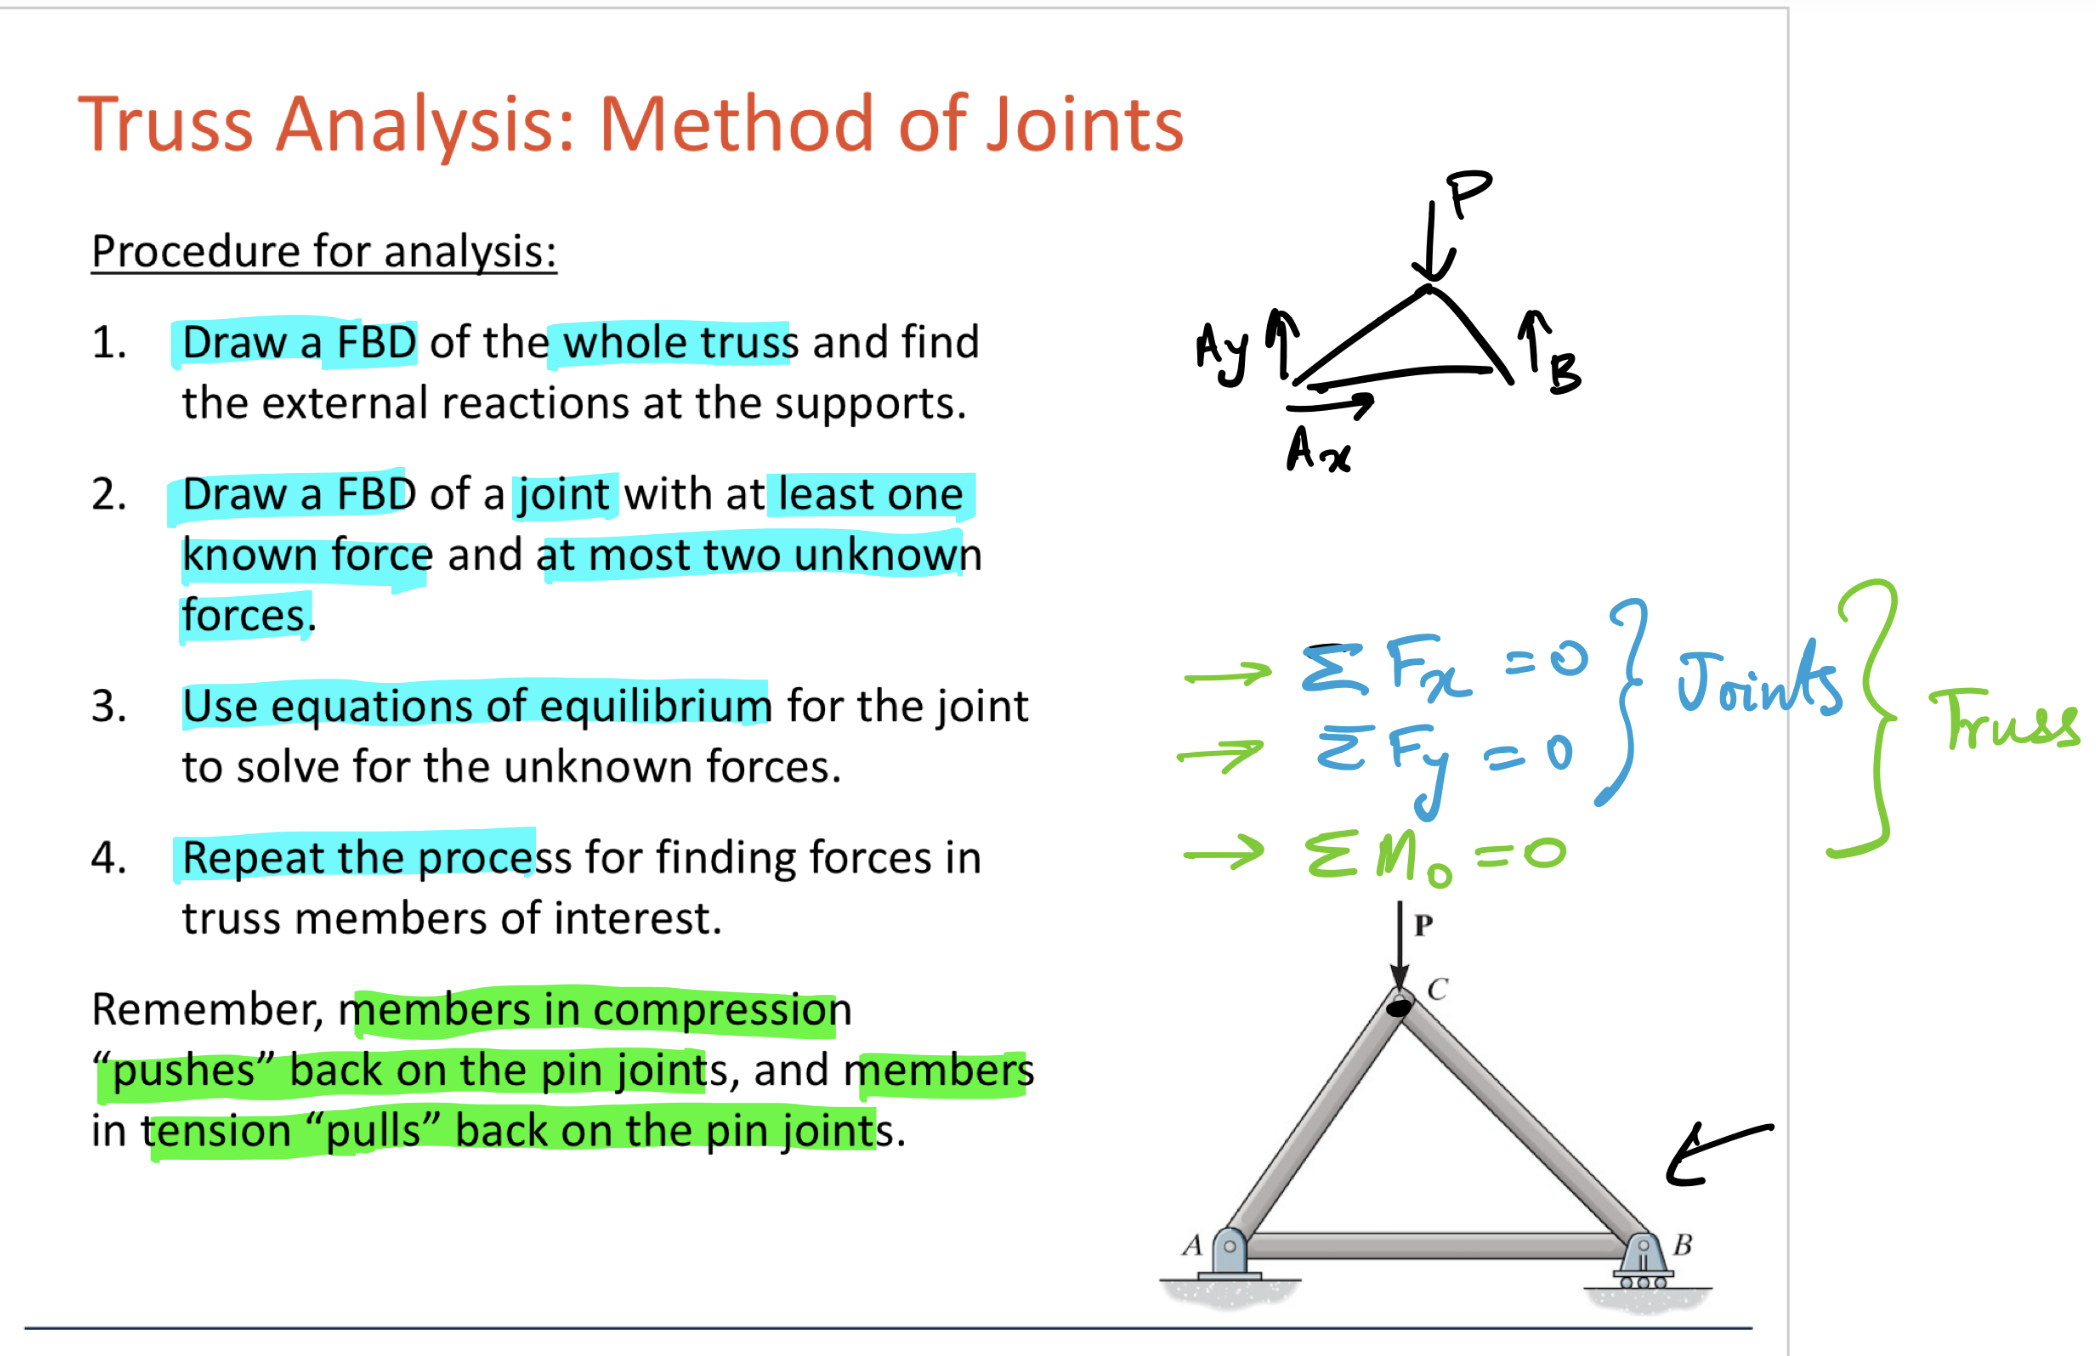
\includegraphics[angle=0, width=5in]{TrussFigures/MethodofJoints.png}
\vspace{-2mm}
\caption{\small \blue{Taken from TAM 210 Lecture 17 notes}}
\vspace{-3mm}
\label{Fig:MethodofJoints}
\end{figure*}

\subsection{Truss Analysis: Sections}

\begin{figure*}[!h]
\centering
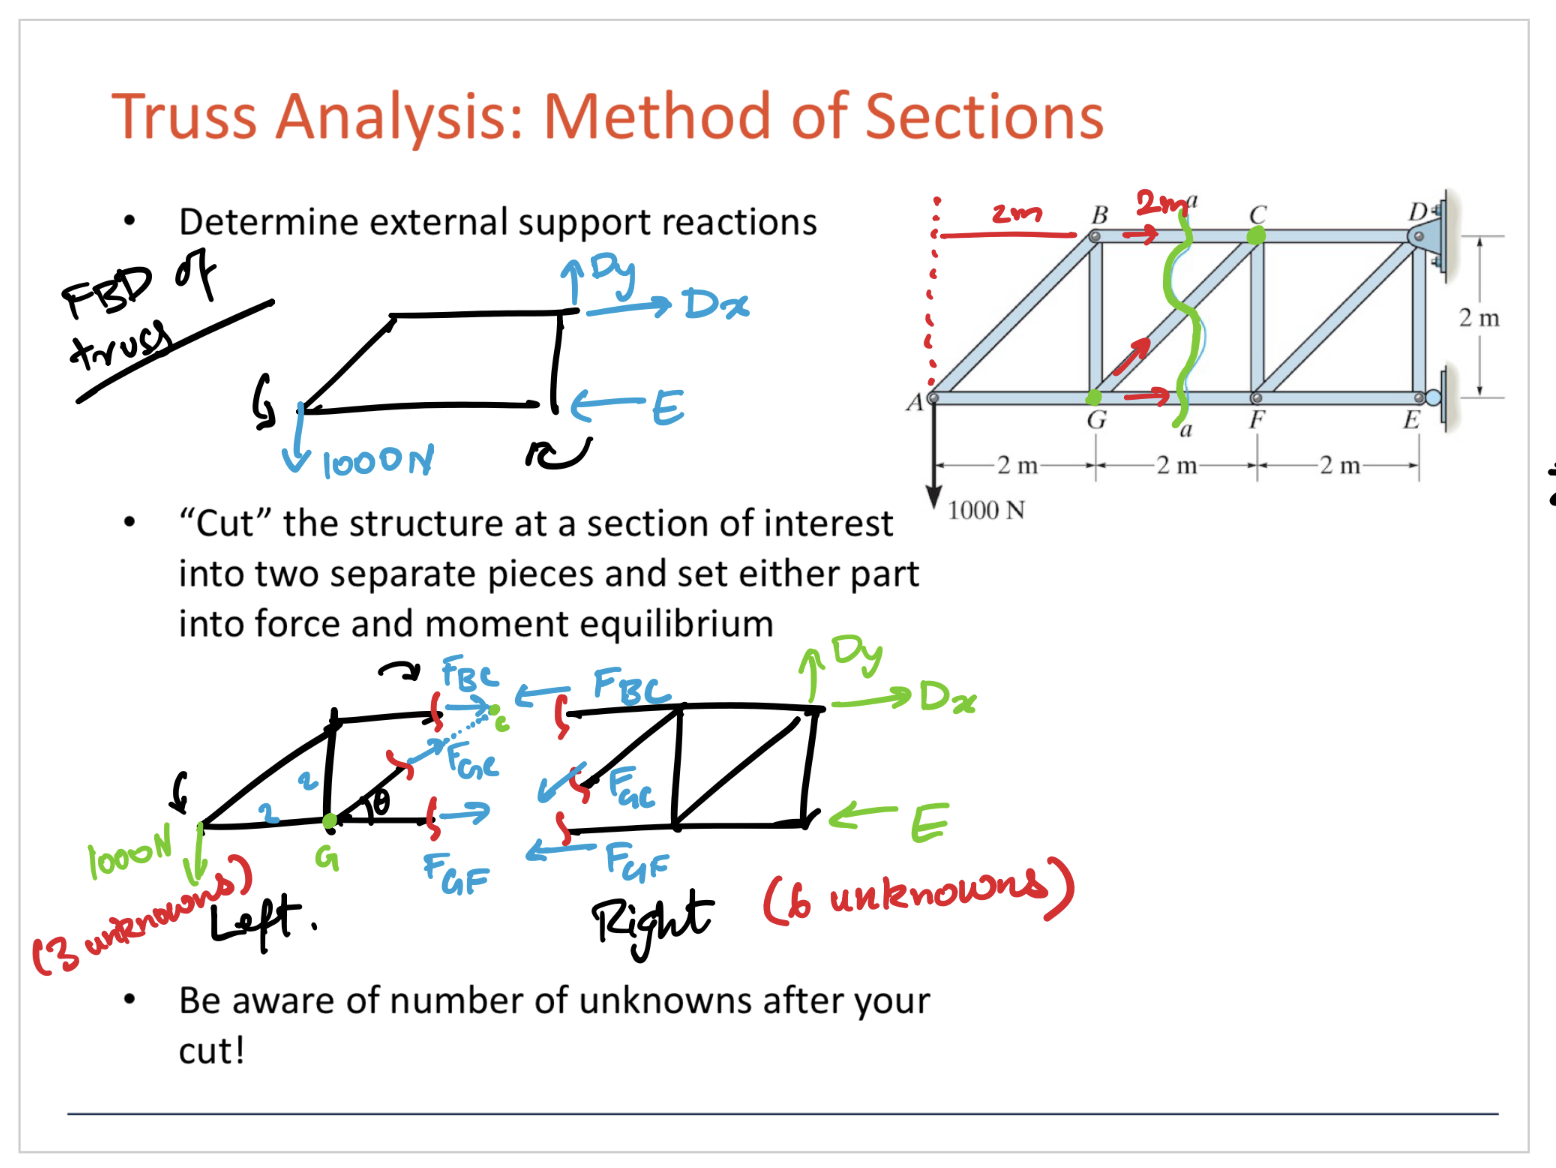
\includegraphics[angle=0, width=5in]{TrussFigures/MethodofSections.png}
\vspace{-2mm}
\caption{\small \blue{Taken from TAM 210 Lecture 19 notes}}
\vspace{-3mm}
\label{Fig:MethodofSections}
\end{figure*}

%lecture 19 




\section{Friction}

Friction is a force that resists the movement of two contacting surfaces sliding relative to each other. Frictional forces act tangential to the surface at the point of contact and act in opposition to the possible or existing motion between the surfaces. 

\blue{Insert content from the TAM 212 page Friction and Damping - Introductory equation box}

\subsection{\red{Static Friction}}

Examples of coefficients of static friction: 

\begin{figure*}[!h]
\centering
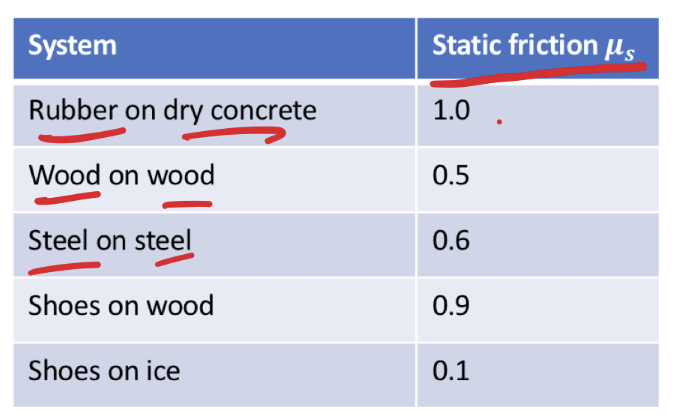
\includegraphics[angle=0, width=3 in]{FrictionFigures/ExampleCoeff.png}
\vspace{-2mm}
\caption{\small \blue{Taken from TAM 210 Lecture 26}}
\vspace{-3mm}
\label{Fig:ExampleCoeff}
\end{figure*}

\blue{This might be a good place to add practical examples - maybe how engine brakes use friction? And another thing about how cartilage in your joints has very little friction (like ice on ice!) which allows for joint movement.}

In TAM 210/211, we will focus on dry friction. Dry friction occurs between two surfaces with \textbf{no} lubricating fluid between them. 

Static friction is the friction between two bodies when there is no movement between them. 

\subsection{Tipping vs. Slipping}

\begin{figure*}[!h]
\centering
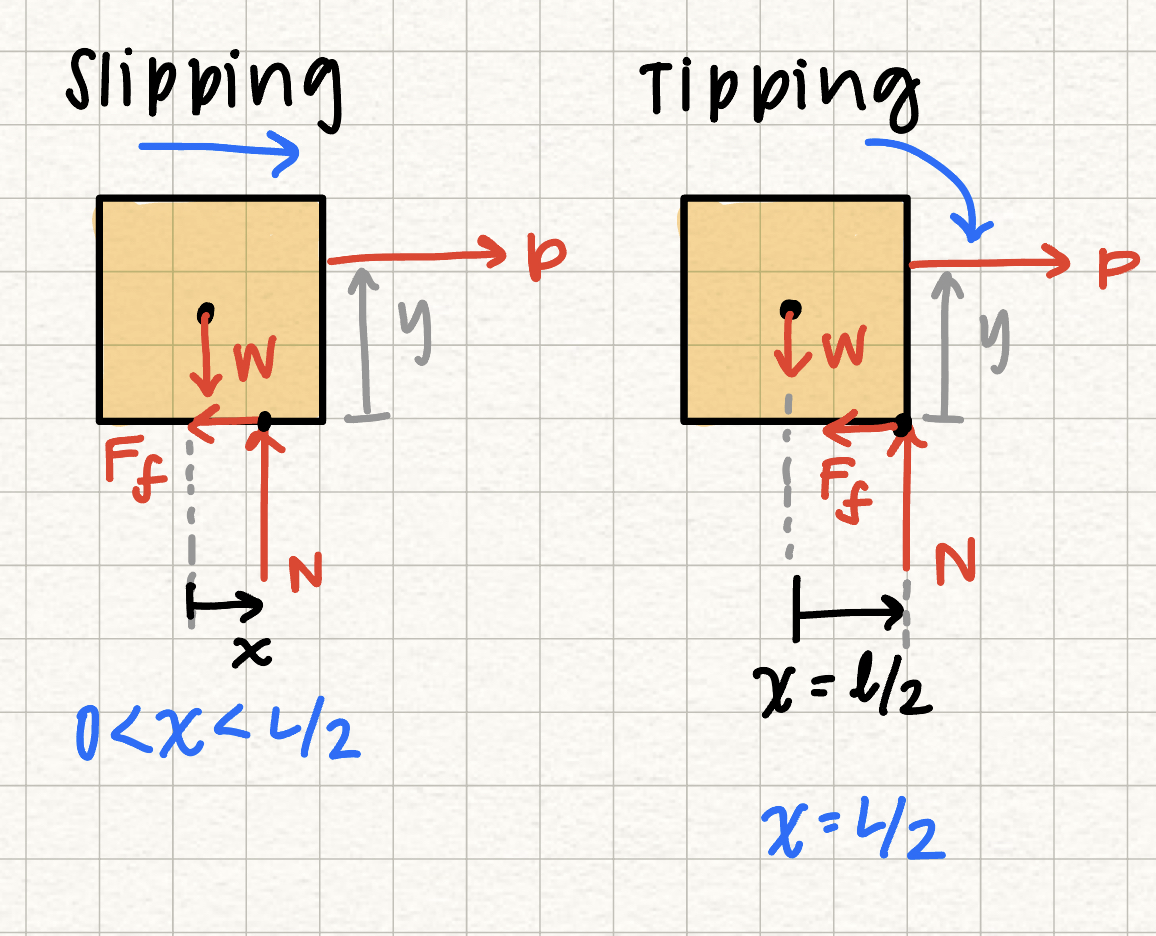
\includegraphics[angle=0, width=\textwidth]{FrictionFigures/TipSlip.png}
\vspace{-2mm}
\caption{\small \blue{Taken from TAM 210 Lecture 27}}
\vspace{-3mm}
\label{Fig:TipSlip}
\end{figure*}

%From Lecture 27


\section{Center of Mass}

\blue{Take from the TAM 212 reference page - Centers of Mass - Introduction section}

%Lectures 28, 29 

\subsection{Basis Shapes}

\blue{Take from the TAM 212 reference page - Centers of Mass - Simplified Shapes}

Centroids of simple shapes can be combined to solve for the centroid of more complex parts. 

\subsection{Centroid}

The centroid denotes the \textit{geometric} center of an object. When an object is made of a homogeneous material, the centroid and the center of mass are at the same point. If the object has an axis of symmetry, the centroid is on the axis of symmetry. In some cases, the centroid may not be on the object. 

\blue{Should we include an example problem from lecture 28?}

\begin{figure*}[!h]
\centering
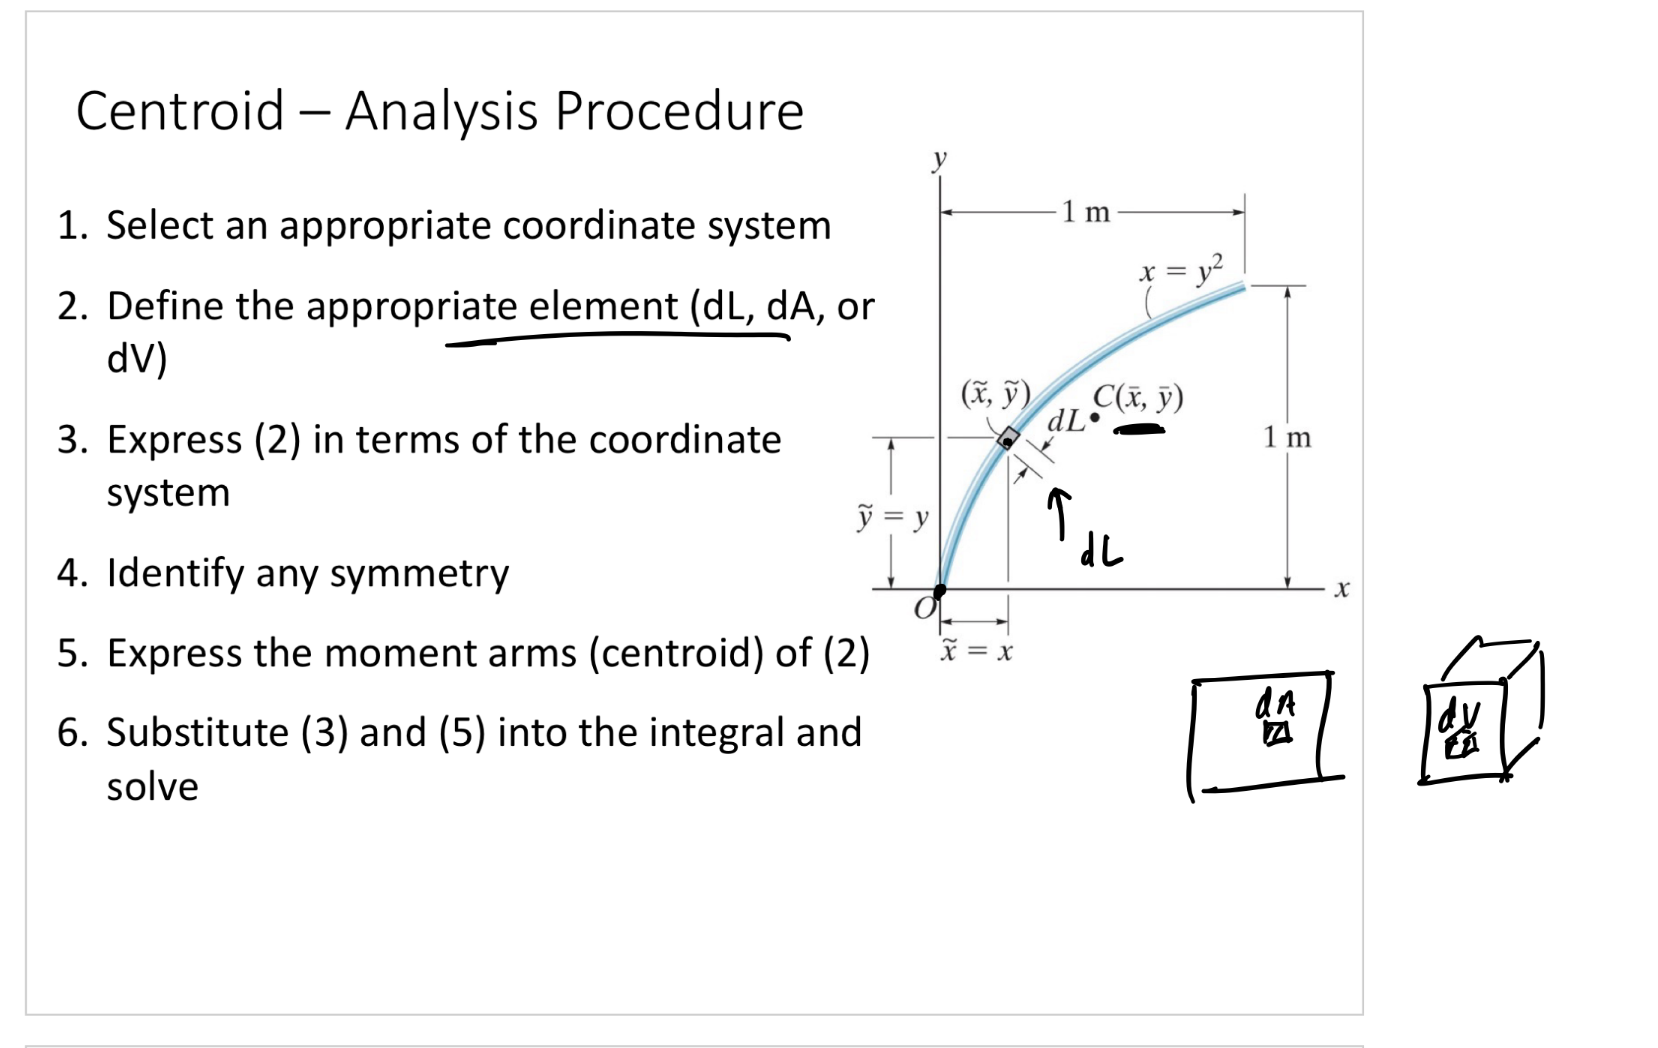
\includegraphics[angle=0, width=5 in]{COMFigures/CentroidAnalysis.png}
\vspace{-2mm}
\caption{\small Nonuniform load. Need to remake this in the same style as the other pictures.}
\vspace{-3mm}
\label{Fig:CentroidAnalysis}
\end{figure*}


\section{Hydrostatic Fluid Pressure}

%Lecture 30, 31, 32
\textbf{Pascal's Law:} A fluid at rest creates a pressure point \textit{p} at a point that is the same in all directions. 

\subsection{Fluid Pressure}

For an incompressible fluid (density $\rho$) at rest, the pressure $p$ varies linearly with fluid depth $z$. This means that the pressure along a horizontal plane (at a certain depth $z$ is constant.

\begin{figure*}[!h]
\centering
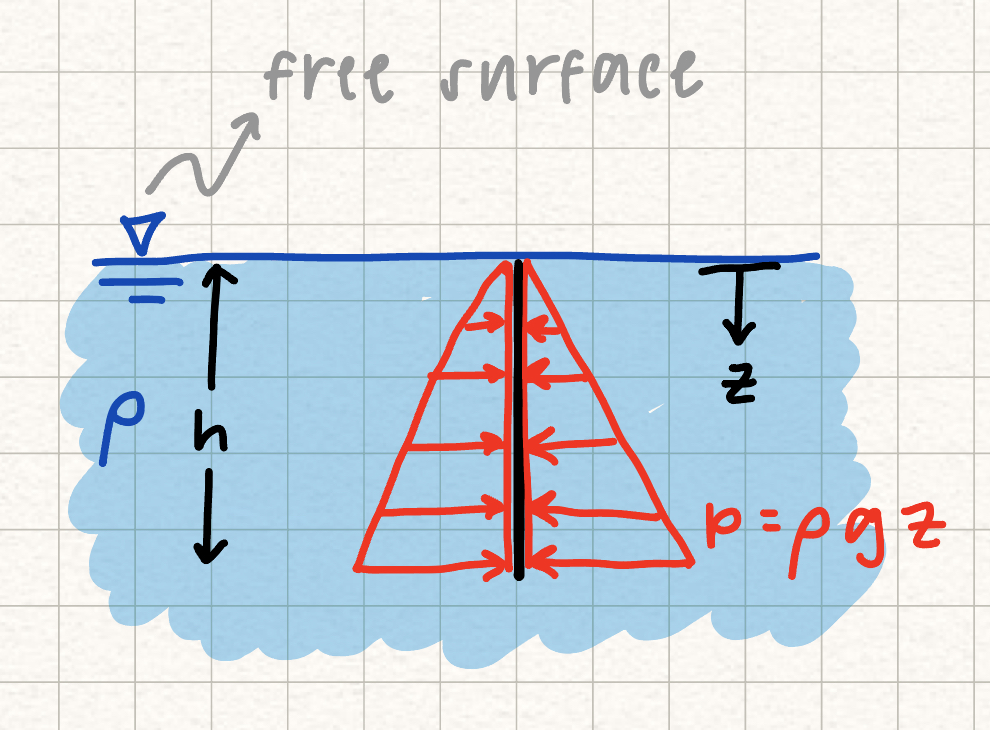
\includegraphics[angle=0, width=4in]{FluidFigures/HydrostaticPressure.jpg}
\vspace{-2mm}
\caption{\small Derivation of the pressure $P(z)$ at the bottom of a cylinder of liquid with cross-sectional area $A$}
\vspace{-3mm}
\label{Fig:HydrostaticPressure}
\end{figure*}

The fluid pressure $P(z)$ can be written as: 

\[P(z) = \rho*g*z\]

\noindent Derivation: 

\begin{figure*}[!h]
\centering
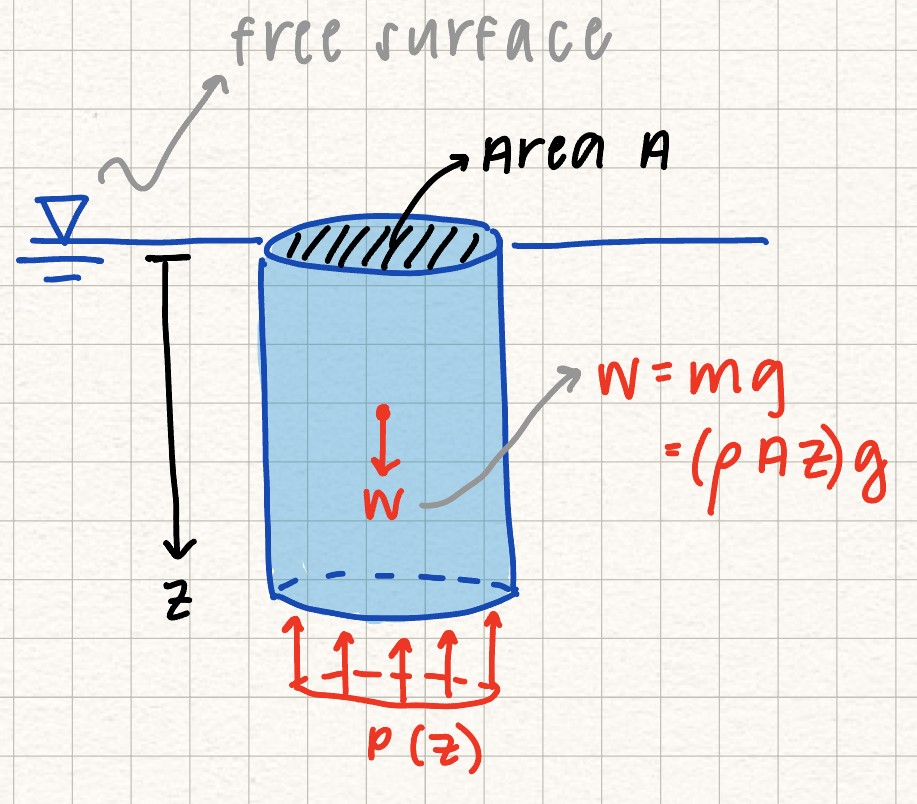
\includegraphics[angle=0, width=\textwidth]{FluidFigures/FluidDerivation.jpg}
\vspace{-2mm}
\caption{\small Derivation of the pressure $P(z)$ at the bottom of a cylinder of liquid with cross-sectional area $A$}
\vspace{-3mm}
\label{Fig:FluidDerivation}
\end{figure*}

\subsection{Buoyancy}

\textbf{Archimedes' Principle:} Any object that is either partially or totally immersed in a fluid has a buoyancy force equal to the weight of the fluid displaced by the object. 


\blue{Do we need to include anything else for buoyancy?}
%Lecture 32
\section{Moment of Inertia}

%Lecture 33
\textit{Note that in statics we are using the second moment of area as our moment of inertia. In dynamics a different moment of inertia is used (the mass moment of inertia). The differences between these two quantities are summarized in the table below: }

\begin{table}[]
\centering
\begin{tabular}{c|c|c}
 & \textbf{Mass moment of inertia} & \textbf{Area moment of inertia} \\ \hline
\textbf{Other names} &  & Second moment of area \\
 &  &  \\
\textbf{Description} & \begin{tabular}[c]{@{}c@{}}Determines the torque \\ needed to produce a \\ desired angular rotation \\ about an axis of rotation \\ (resistance to rotation)\end{tabular} & \begin{tabular}[c]{@{}c@{}}Determines the moment \\ needed to produce a \\ desired curvature \\ about an axis \\ (resistance to bending)\end{tabular} \\
 &  &  \\
\textbf{Equations} & 
\begin{tabular}[c]{@{}c@{}} 
 \[I_{P,\hat{a}} = \iiint_\mathcal{B} \rho r^2 \,dV\] \\ 
 \end{tabular} &

 \begin{tabular}[c]{@{}c@{}}
 \[I_x = \int_{A}^{} y^2 \,dA \]\\ 
 \[I_y = \int_{A}^{} x^2 \,dA \]\\ 
 \[J_O = \int_{A}^{} r^2 \,dA = \int_{A}^{} (x^2+y^2) \,dA\]
 \end{tabular} \\
 
 &  \\
\textbf{Units} & length*mass\textasciicircum{}2 & length\textasciicircum{}4 \\
 &  &  \\
\textbf{Typical Equations} & \[\tau = I\alpha \] &  \[\sigma = (My)/I \]\\
 &  &  \\
\textbf{Courses} & TAM 212 & TAM 210, TAM 251
\end{tabular}
\end{table}

\subsection{Moment of Inertia (Second Moment of Area)}

The moment of inertia used in statics is the "second moment of area", which is a mass property that determines the amount of torque that is needed to create an angular acceleration about a specific axis of rotation. The dimension of the area moment of inertia is $length^4$.\\

Moment of inertia about the x-axis:  \[I_x = \int_{A}^{} y^2 \,dA \]

Moment of inertia about the y-axis: \[I_y = \int_{A}^{} x^2 \,dA \]

Polar moment of inertia: \[J_O = \int_{A}^{} r^2 \,dA = \int_{A}^{} (x^2+y^2) \,dA\]
\textit{Note that the polar moment of inertia depicts the measure of the distribution of area about a point (usually the origin), rather than about an axis.}

\subsection{Parallel axis theorum}

\blue{Need to transcribe this to be the correct format and drawings}

\begin{figure*}[!h]
\centering
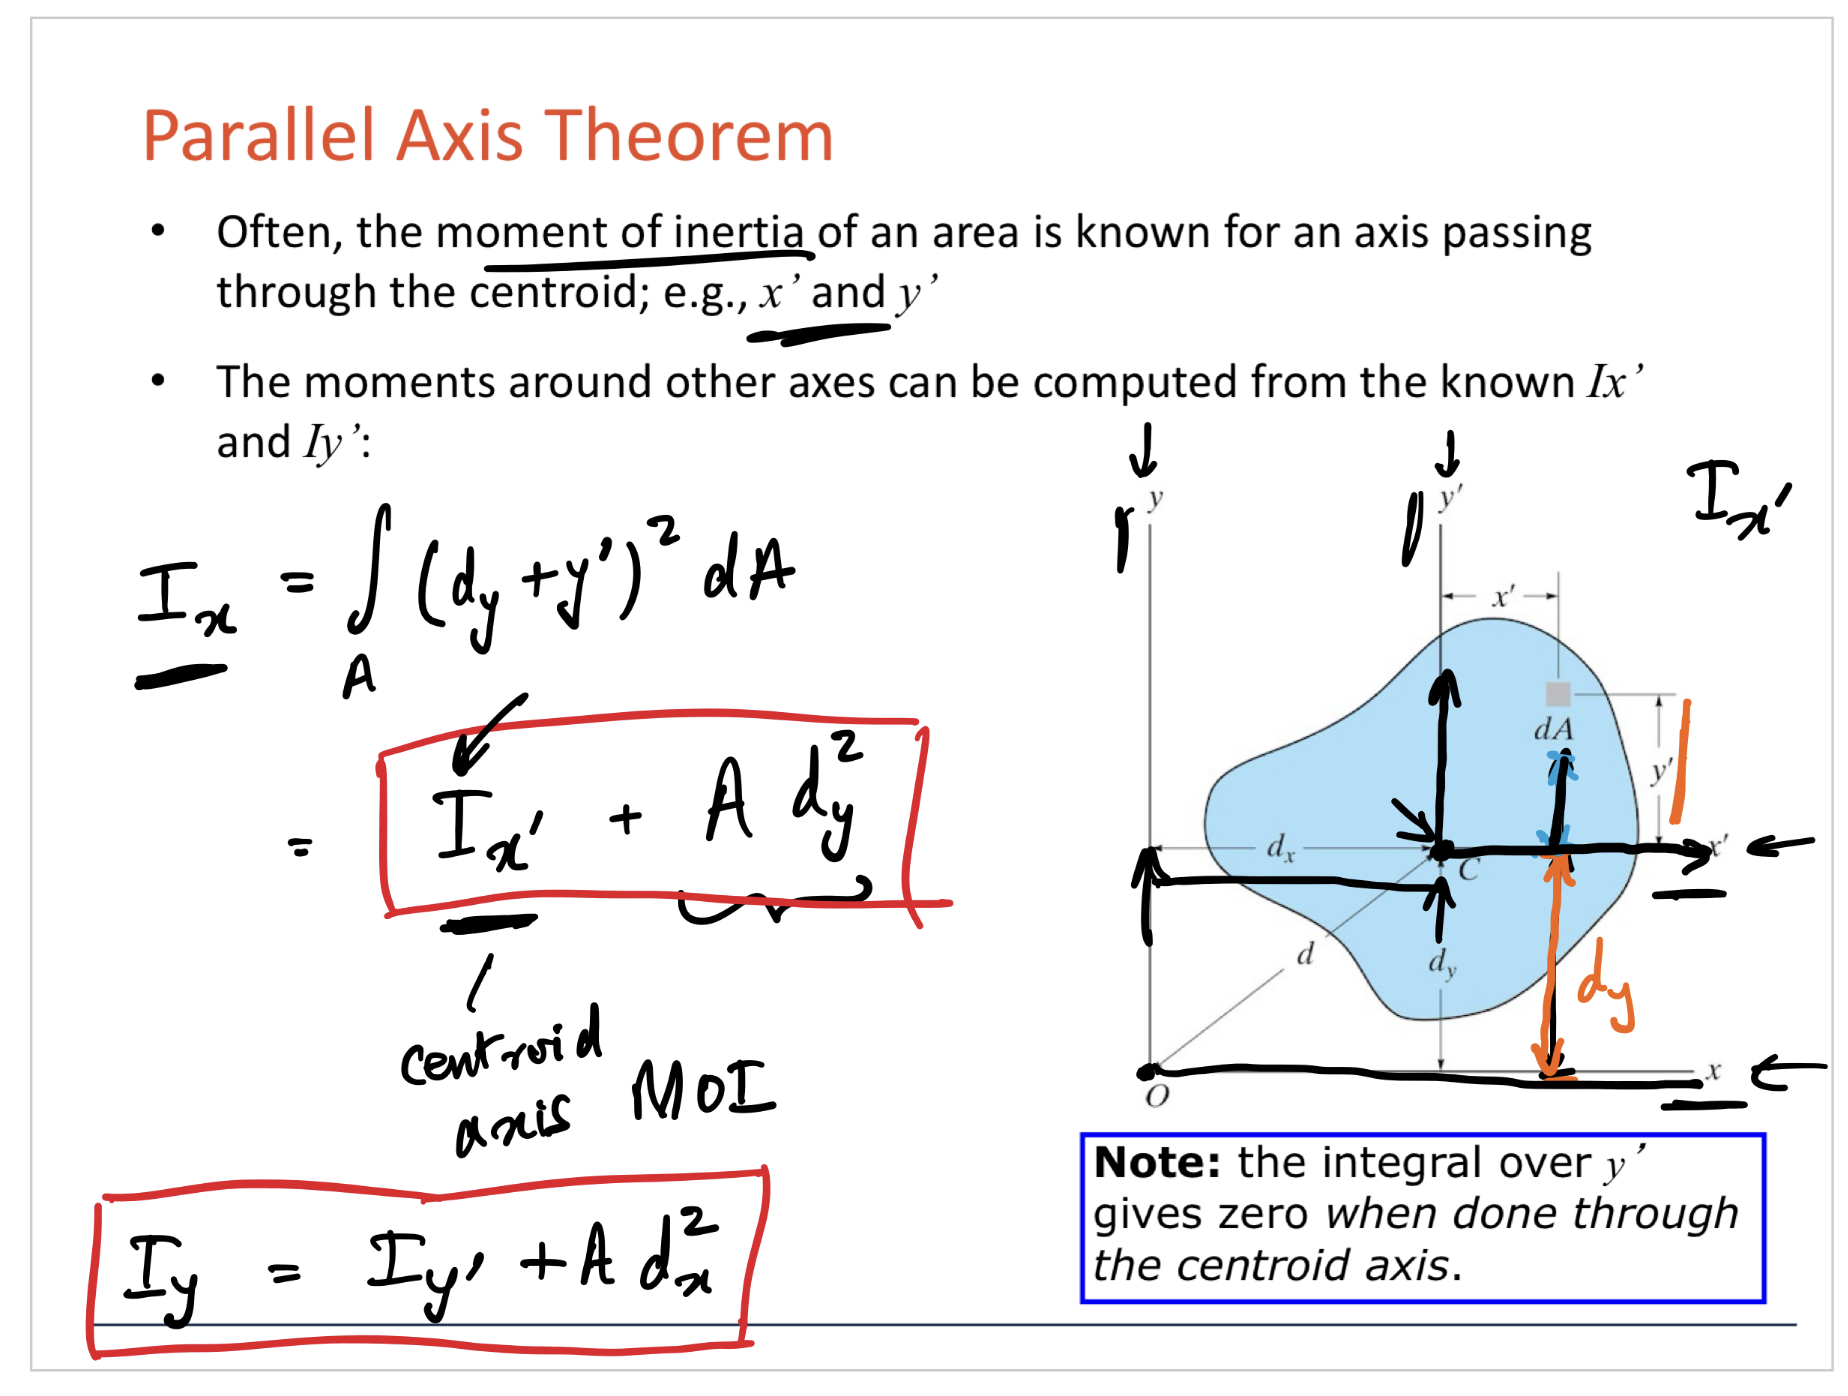
\includegraphics[angle=0, width=\textwidth]{MOIFigures/ParallelAxisThm.png}
\vspace{-2mm}
\caption{\small \blue{Taken from TAM 210 Lecture 3 - Slide 3}}
\vspace{-3mm}
\label{Fig:ParallelAxisThm}
\end{figure*}


\subsection{Combining moments of inertia}

\blue{Need to transcribe this to be the correct format and drawings - show the example problem with the house-shaped object.}

\begin{figure*}[!h]
\centering
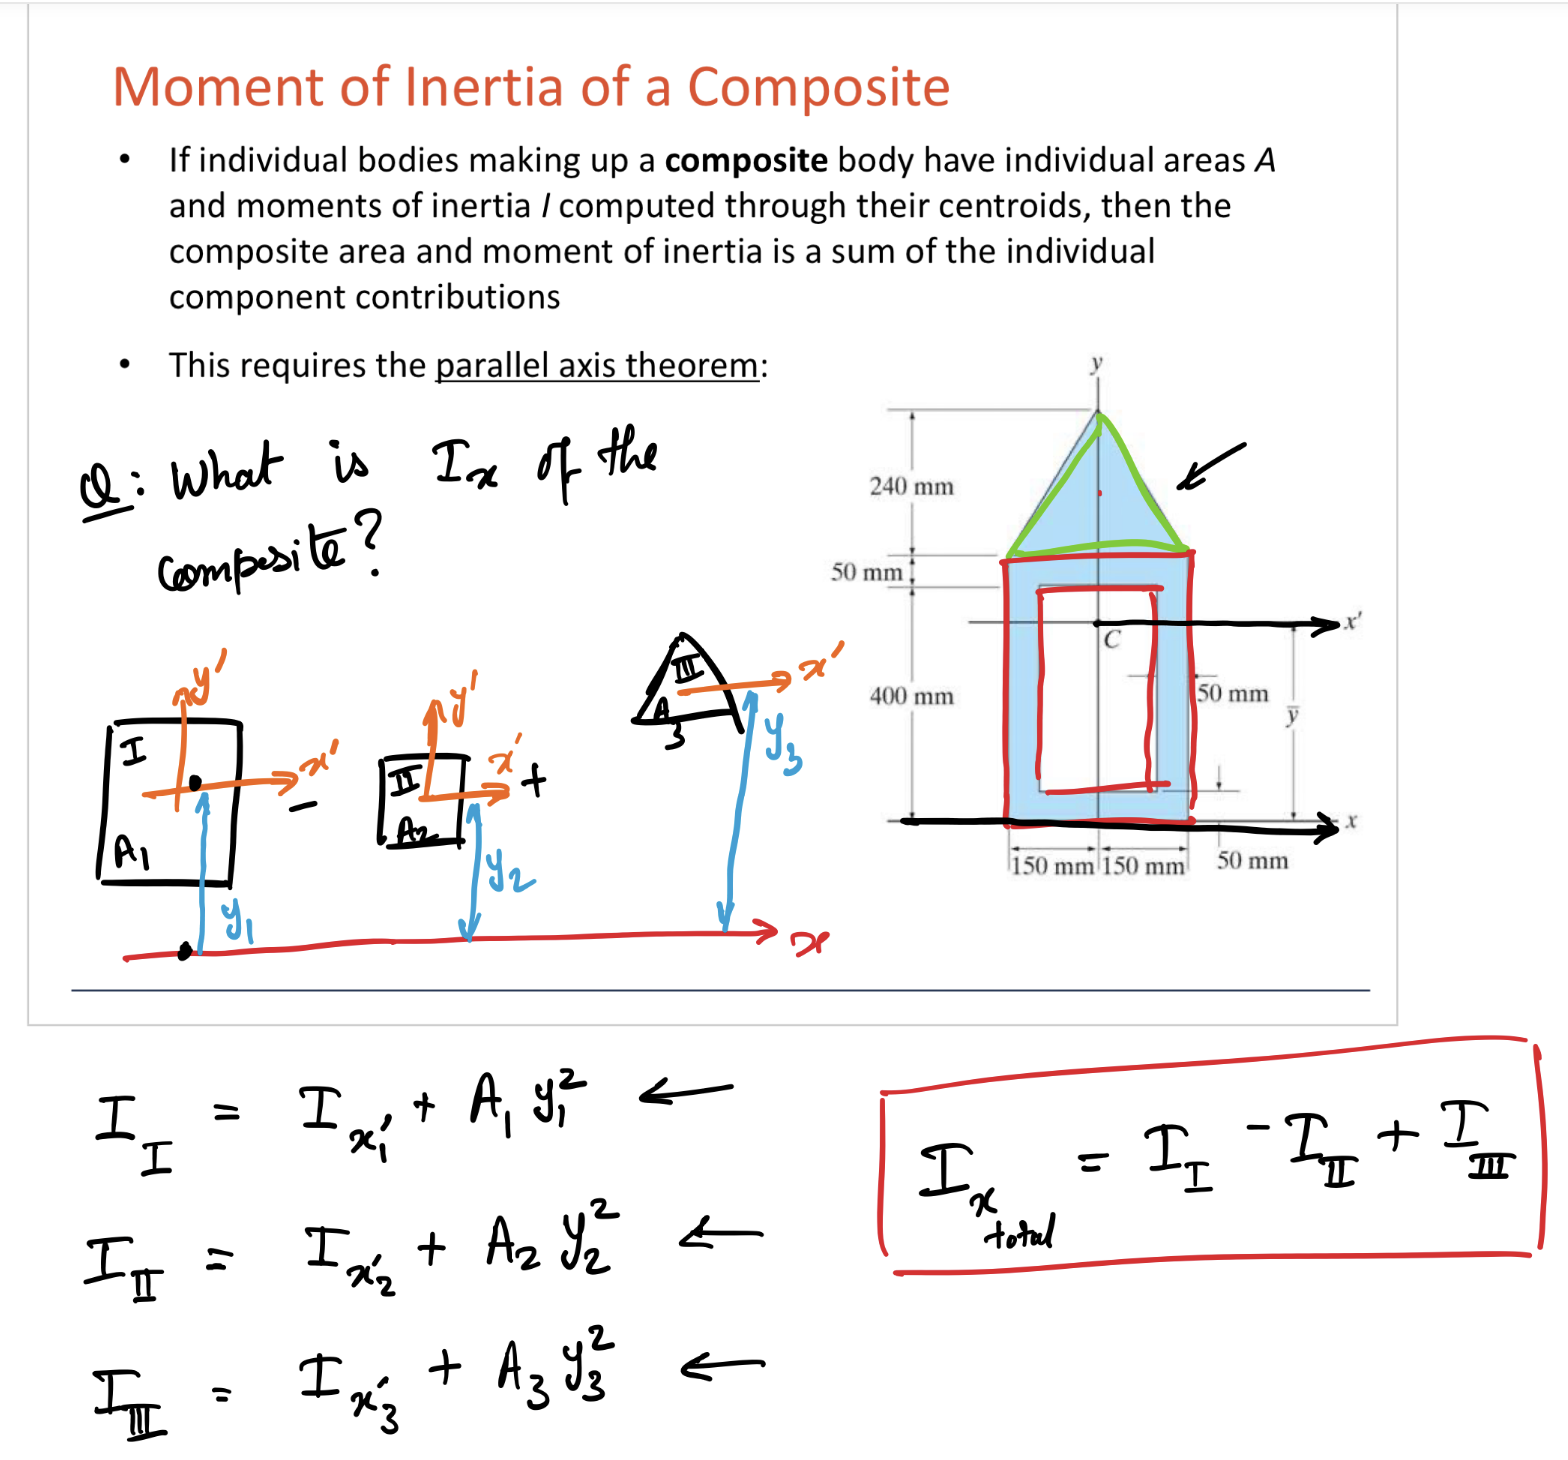
\includegraphics[angle=0, width=\textwidth]{MOIFigures/MOIComposite.png}
\vspace{-2mm}
\caption{\small \blue{Taken from TAM 210 Lecture 3 - Slide 3}}
\vspace{-3mm}
\label{Fig:MOIComposite}
\end{figure*}

\subsection{Moment of inertia for typical shapes}

\begin{figure*}[!h]
\centering
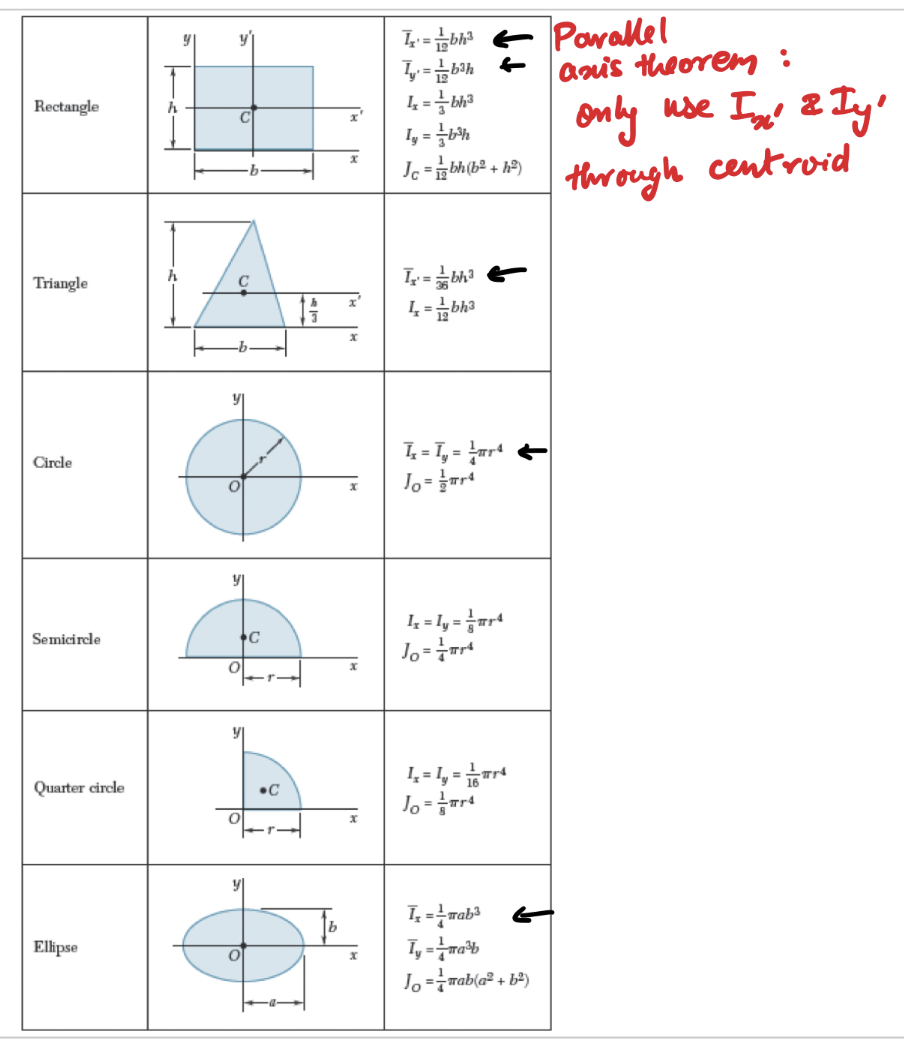
\includegraphics[angle=0, width=\textwidth]{MOIFigures/TypicalMOI.png}
\vspace{-2mm}
\caption{\small \blue{Taken from TAM 210 Lecture 3 - Slide 3}}
\vspace{-3mm}
\label{Fig:TypicalMOI}
\end{figure*}


\section{Virtual Work}

%Lectures 34 and 35
A force does work when it produces a displacement along its line of action. 

Virtual work ($dU$) is the work produced by a force over an infinitesimally small displacement $dr$.

\[dU = F\cdot dr\]

Virtual work of a couple moment: 

\[dU = \Vec{M}\cdot d\theta \Vec{k}\]

\begin{figure*}[!h]
\centering
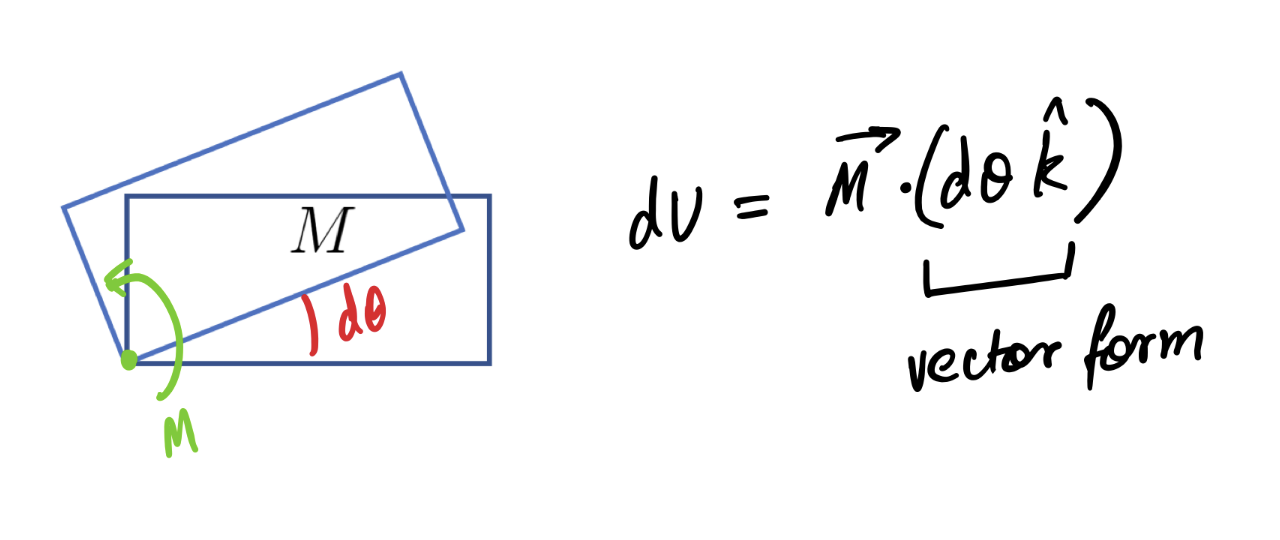
\includegraphics[angle=0, width=5 in]{VWorkFigures/VWorkCoupleMoment.png}
\vspace{-2mm}
\caption{\small Virtual work $dU$ completed by a couple moment, $M$. \blue{Need to add a coordinate system to this picture. Taken from lecture 34.}}
\vspace{-3mm}
\label{Fig:VWorkCoupleMoment}
\end{figure*}

We can use virtual work to solve for the forces in a system without needing to solve for all of the support reactions. For example, if a truss is completely pinned on one end, it doesn't move, which means there is no virtual work completed on that pin because there are no virtual displacements!

\subsection{Virtual displacements}
A virtual displacement is an infinitesimally small displacement (or rotation) that is possible in the system, denoted usually as $dx$ or $d\theta$. It's important to note that virtual displacements are assumed to be possible but don't actually exist. 

\subsection{Principle of Virtual Work}

If a body is in equilibrium, the sum of the virtual work done by all the forces and couple moments acting on the body is zero. 

\begin{figure*}[!h]
\centering
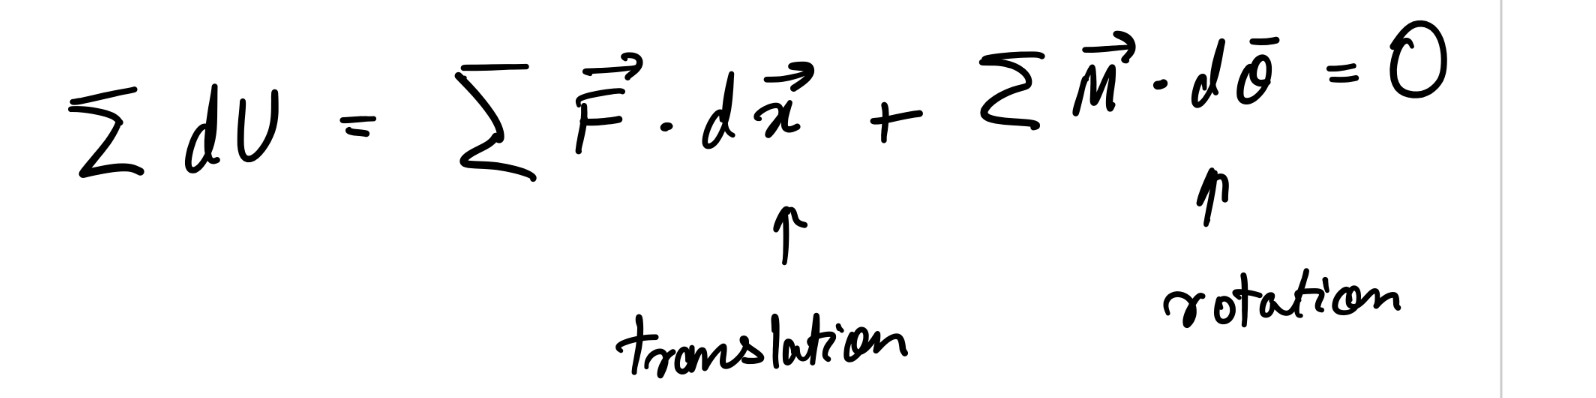
\includegraphics[angle=0, width=5 in]{VWorkFigures/PVW.png}
\vspace{-2mm}
\caption{\small Principle of virtual work. \blue{Taken from lecture 34.}}
\vspace{-3mm}
\label{Fig:PVW}
\end{figure*}

\subsection{Virtual work analysis}

\begin{figure*}[!h]
\centering
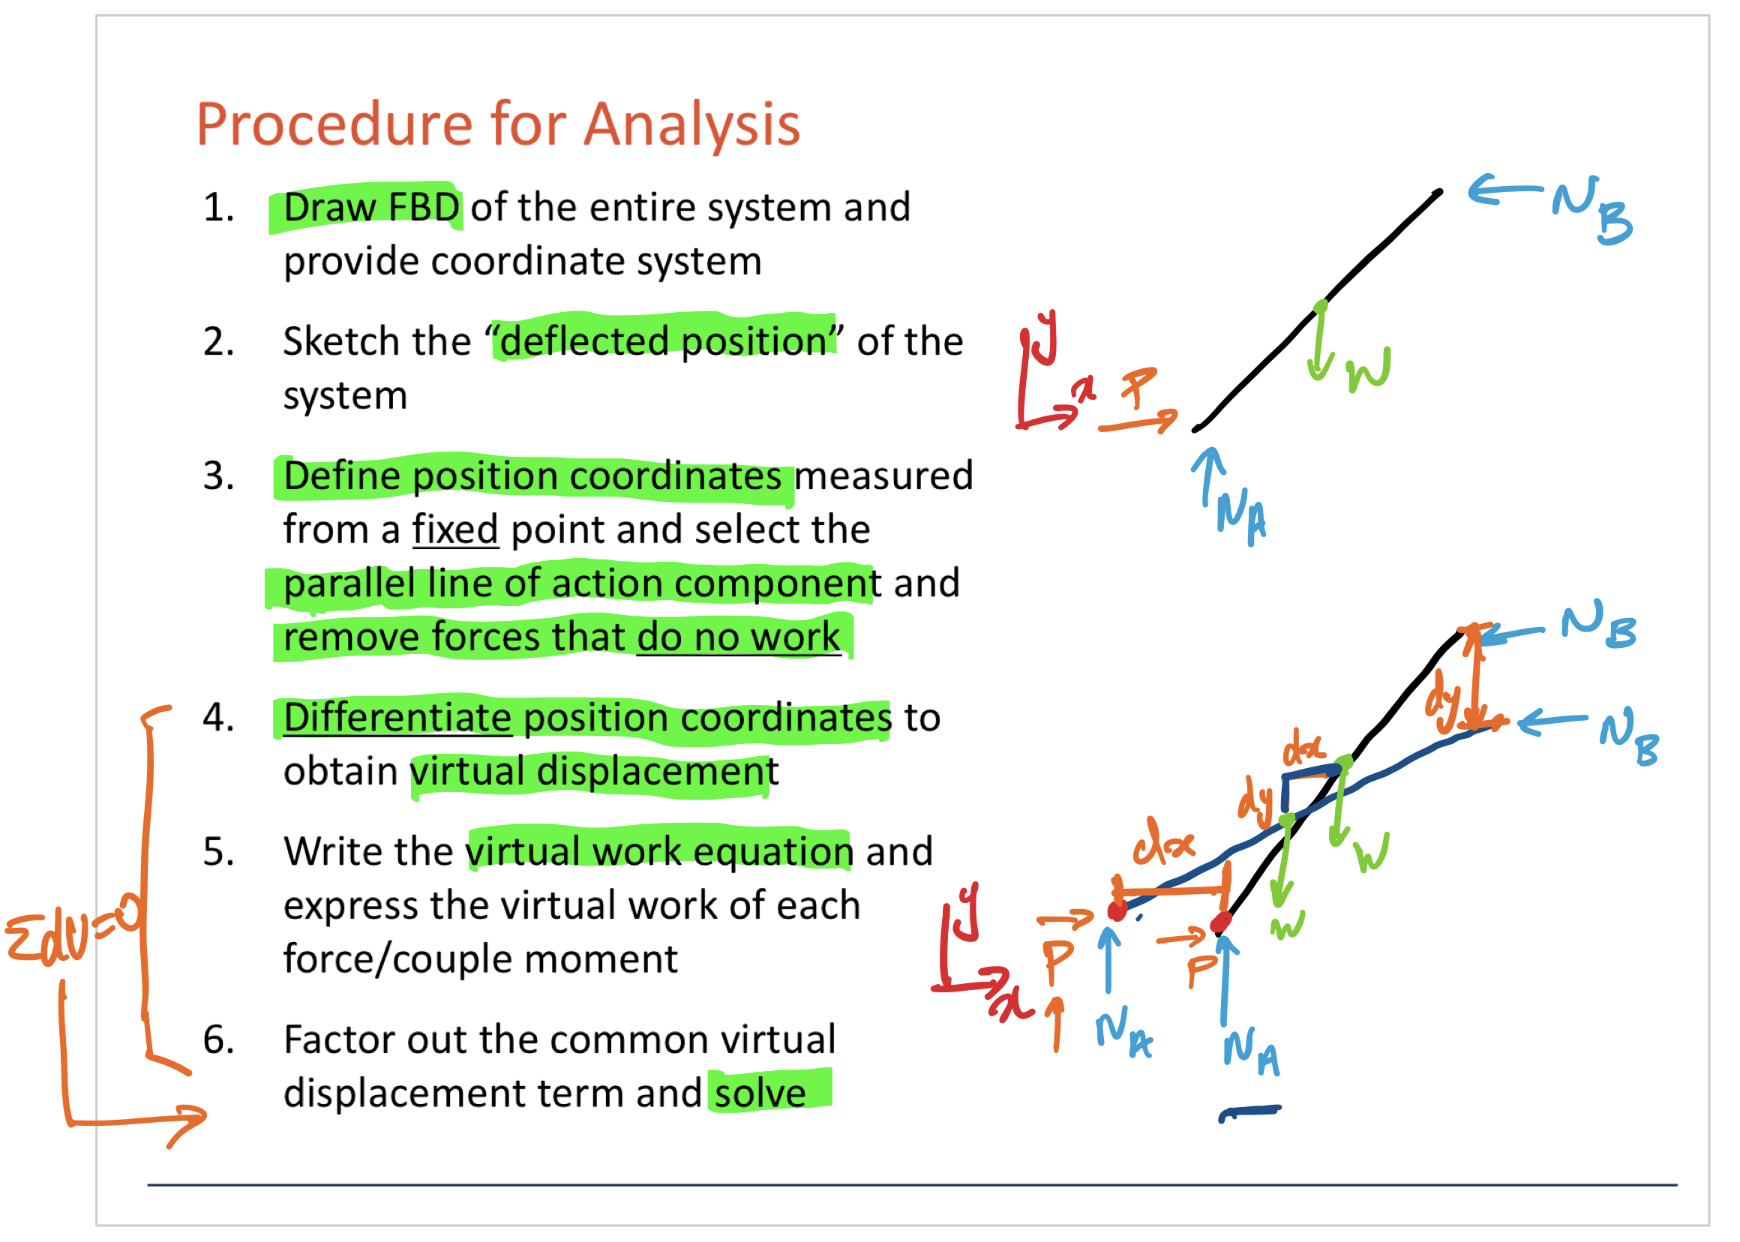
\includegraphics[angle=0, width=5 in]{VWorkFigures/VWAnalysis.png}
\vspace{-2mm}
\caption{\small Analysis procedure for virtual work problems. \blue{Taken from lecture 34.}}
\vspace{-3mm}
\label{Fig:PVW}
\end{figure*}

\end{document}
